%%%%%%%%%%%%%%%%%%%%%%%%%%%%%%%%%%%%%%%%% 
% University/School Laboratory Report
% LaTeX Template
% Version 3.1 (25/3/14)
% 
% This template has been downloaded from:
% http://www.LaTeXTemplates.com
% 
% Original author:
% Linux and Unix Users Group at Virginia Tech Wiki 
% (https://vtluug.org/wiki/Example_LaTeX_chem_lab_report)
% 
% License:
% CC BY-NC-SA 3.0 (http://creativecommons.org/licenses/by-nc-sa/3.0/)
% 
%%%%%%%%%%%%%%%%%%%%%%%%%%%%%%%%%%%%%%%%% 

% ----------------------------------------------------------------------------------------
%	PACKAGES AND DOCUMENT CONFIGURATIONS
% ----------------------------------------------------------------------------------------

\documentclass{article}

\usepackage{graphicx} % Required for the inclusion of images
\usepackage{epstopdf} % eps to pdf
\usepackage{epsfig}
\usepackage{amsmath} % Required for some math elements 
\usepackage{hyperref}
\usepackage{algorithm}
\usepackage{algpseudocode}
\usepackage{tikz}
\usepackage{pgflibraryarrows}
\usepackage{pgflibrarysnakes}
\usepackage{subfig}
\usepackage{booktabs} 
\newtheorem{remark}{Remark}[section]
% \setlength\parindent{0pt} % Removes all indentation from paragraphs

% \renewcommand{\labelenumi}{\alph{enumi}.} % Make numbering in the enumerate environment by letter rather than number (e.g. section 6)

% \usepackage{times} % Uncomment to use the Times New Roman font

% ----------------------------------------------------------------------------------------
%	DOCUMENT INFORMATION
% ----------------------------------------------------------------------------------------

\title{The Unsteady Navier-Stokes Flow Using Adaptive Mixed Finite Elements
} % Title

\author{Yirong Wu and Heyu Wang \\
  \small Department of Mathematics, ZheJiang University, HangZhou,
  310027, China\\
  \small Department of Mathematics, ZheJiang University, HangZhou,
  310027, China }
% Author name
% \date{\today} % Date for the report

\begin{document}

\maketitle % Insert the title, author and date

% \begin{center}
%   \begin{tabular}{l r}
%     Date Performed: & April 28, 2014 \\ % Date the experiment was performed
%     Partners: & Heyu Wang \\ % Partner names
%     %     & Peter Jim \\
%     Instructor: & Professor Heyu Wang \\% Instructor/supervisor
%     Address: & Department of Mathematics, ZheJiang University 
%   \end{tabular}
% \end{center}

% If you wish to include an abstract, uncomment the lines below
% \begin{abstract}
%   Abstract text
% \end{abstract}

% ----------------------------------------------------------------------------------------
%	SECTION 1
% ----------------------------------------------------------------------------------------
\begin{abstract}
\end{abstract}
% ----------------------------------------------------------------------------------------
%	SECTION 2
% ----------------------------------------------------------------------------------------
\section{Accuracy Solution}
The Navier-Stokes equations:
\begin{equation}
  \begin{array}{rcl}
    \frac{\partial \vec{u}}{\partial t}-\nu \nabla^2 \vec{u} +
    \vec{u} \cdot \nabla \vec{u} + \nabla p & =
    & \vec{0},\\
    \nabla \cdot \vec{u} & = & 0,
  \end{array}
  \label{eq::NS}
\end{equation}
The accuracy solutions of euqations (\ref{eq::NS}) is defined as
follows:
\begin{equation}
  \begin{array}{rcl}
    u(x, y, t) & = & -cos(x)sin(y)e^{-2 \nu t},\\
    v(x, y, t) & = & sin(x)sin(y)e^{-2 \nu t}, \\
    p(x, y, t) & = & \frac{1}{2}(sin^2(x) + sin^2(y)) e^{-4 \nu t} + \text{constant}
  \end{array}
  \label{eq::accuracy_solution}
\end{equation}
with the computing domain $[0, 2 \pi] \times [0, 2 \pi]$.

\section{Numerical result}
\subsection{Uniform mesh}
\subsubsection{Error analysis}
From Table [\ref{tab::accuracy_uniform_error}], we can conclude $L_2$
error of velocity is $O(h^2)$, $H_1$ semierror of velocity is $O(h)$. 
\begin{table}[!htbp]
  \centering
  \begin{tabular}{ccccccc} \toprule
    Mesh (P)  & $||u - u_h ||_{L^2}$ & $||u - u_h ||_{H^1}$ & $||v -
    v_h||_{L^2}$ & $||v - v_h||_{H^1}$ & $||p - p_h||_{L^2}$ & $||p -
    p_h||_{H^1}$ \\ \midrule
    $20 \times 20$ &   $6.734 e{-3}$    & $2.319 e{-1}$ &
    $6.734 e{-3}$   &$2.311 e{-1}$   &   $1.547 
    e{-2}$ &   $4.098  e{-1}$ \\ \midrule
    $40 \times 40$   &   $1.545 e{-3}$   &   $1.131 e{-1}$  &
    $1.535   e{-3}$ & $1.126   e{-1}$ &
    $3.917   e{-3}$ & $2.041   e{-1}$ \\ \midrule
    $80 \times  80$ &   $3.816  e{-4}$   &   $5.642 
    e{-2} $ &  $3.789  e{-4}$ & $5.615  e{-2}$ &
    $6.444   e{-4}$ & $1.019  e{-1}$ \\ \bottomrule
  \end{tabular}
  \caption{\small Error for Accuracy test using uniform mesh, $\nu = 0.05, t = 1s$.}
  \label{tab::accuracy_uniform_error}
\end{table}

\subsubsection{Mesh 20 * 20}

 Steamline of velocity and contour of pressure is shown in Figure (\ref{fig::uniform20_solution}).
 \begin{figure}[ht]
   \centering
   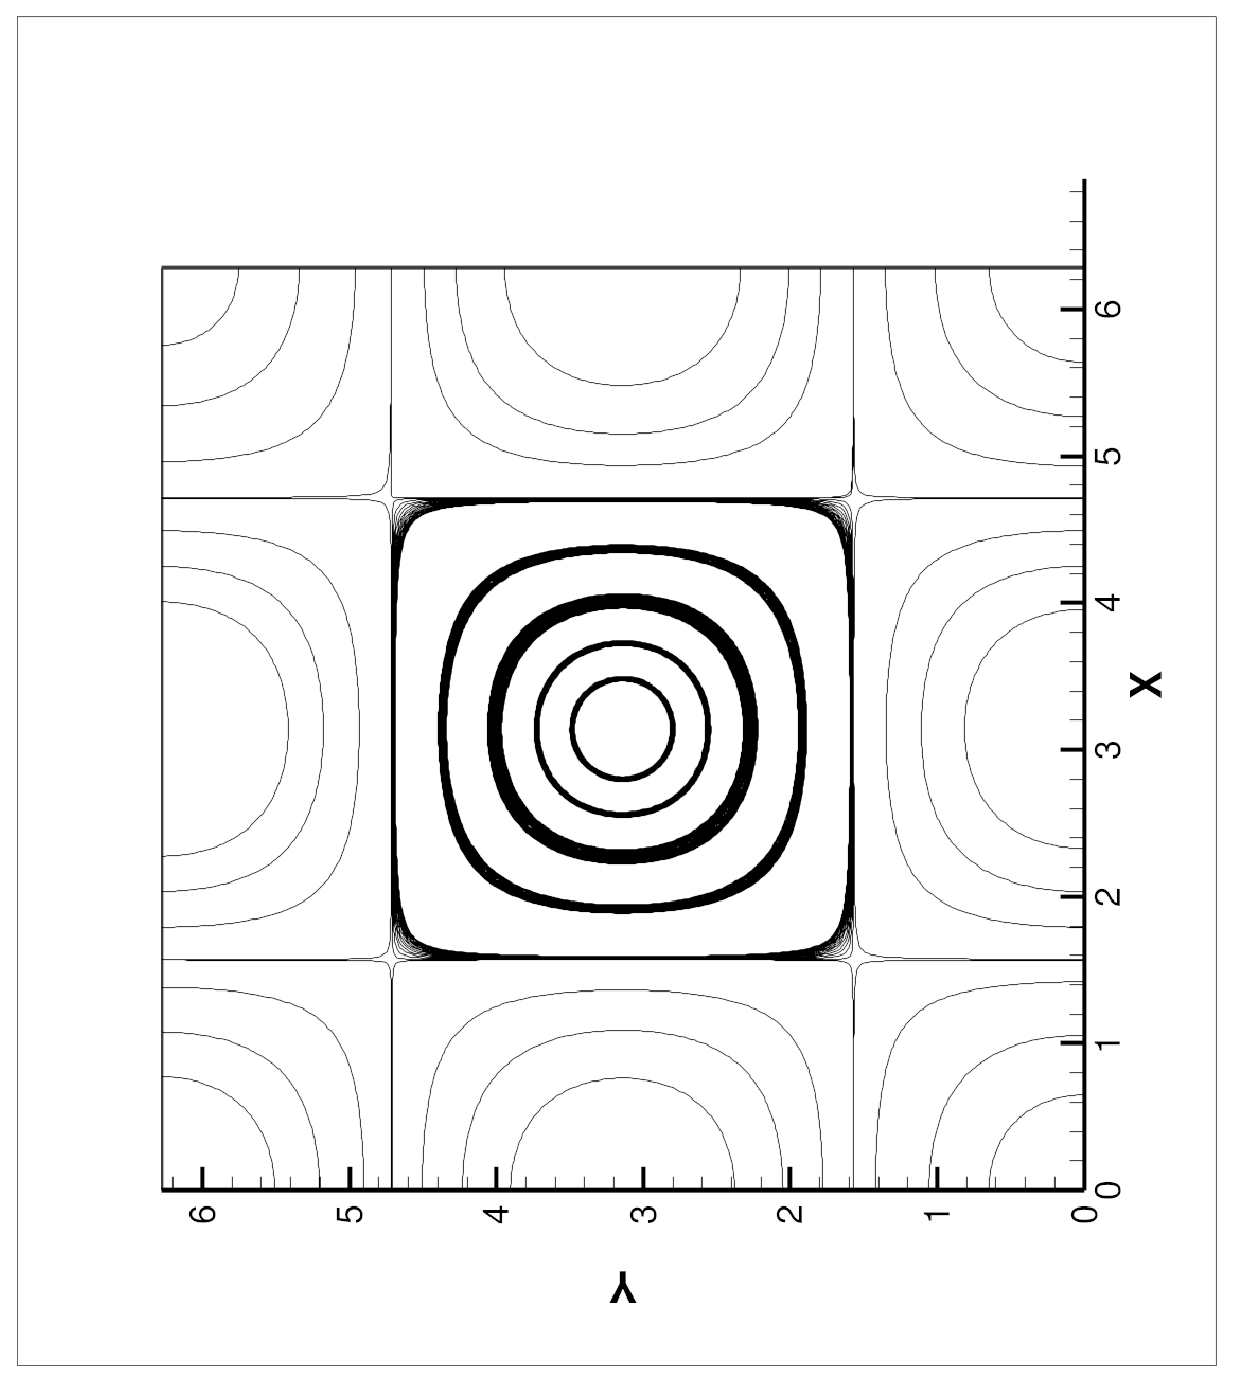
\includegraphics[width = 0.43\textwidth, angle = -90]{./uniform20_streamline.eps}
   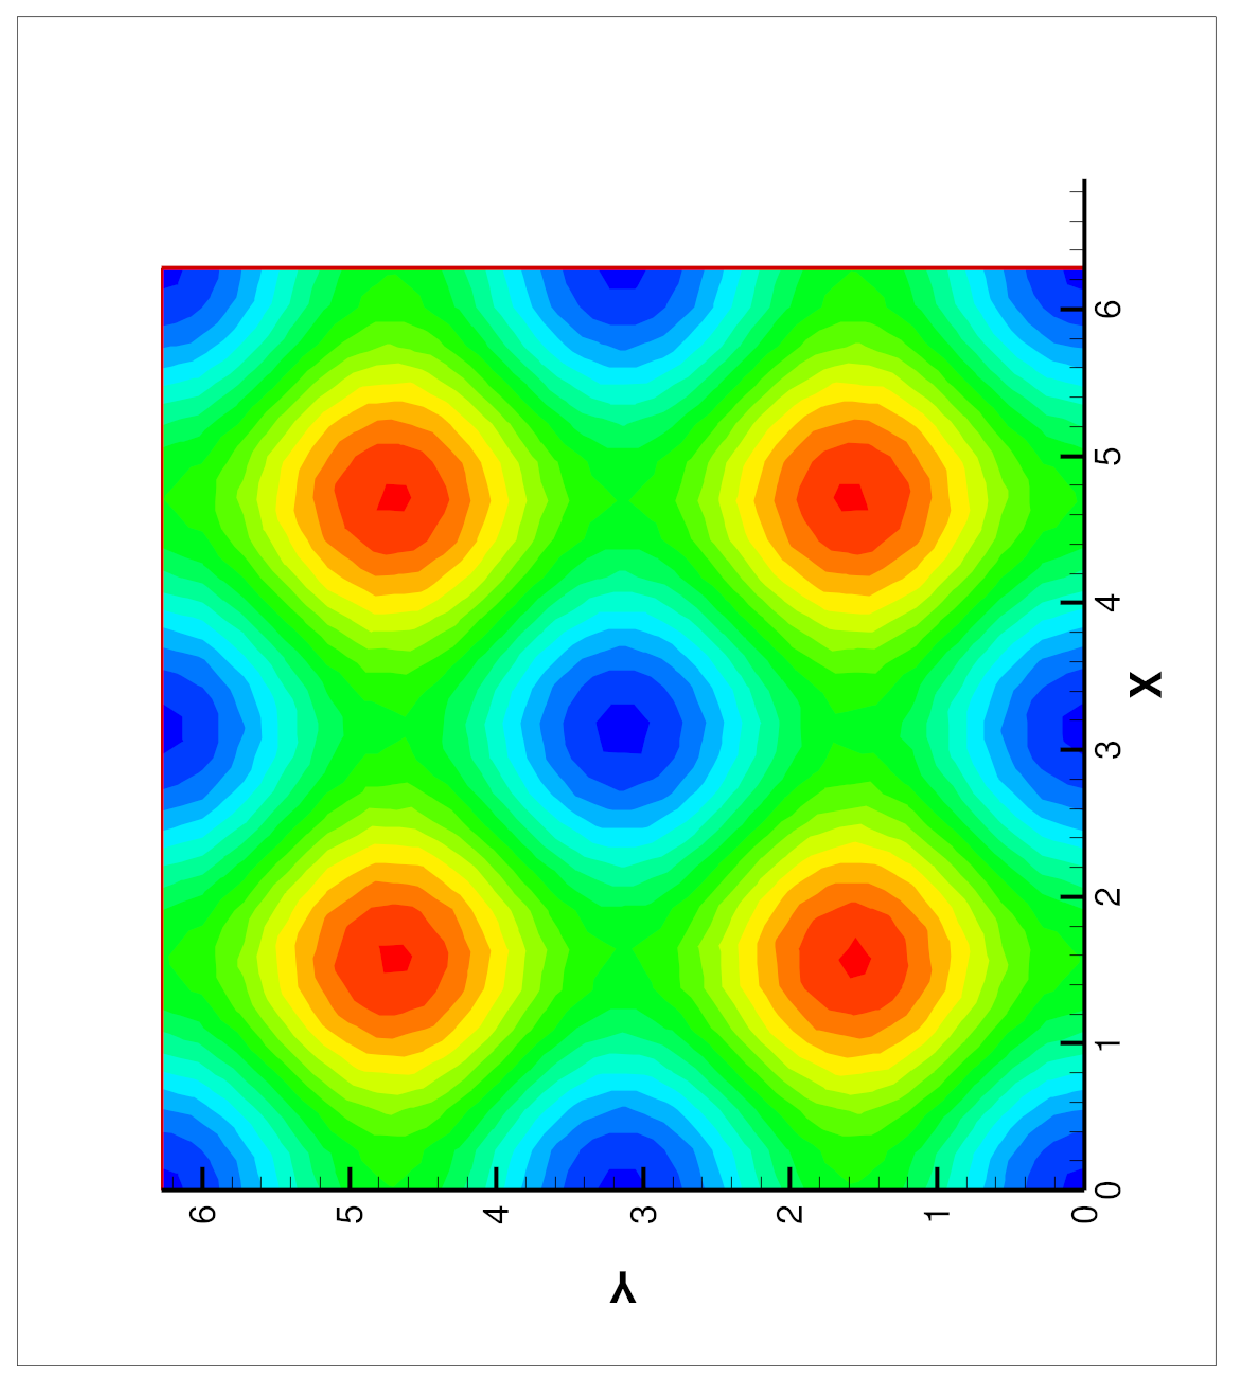
\includegraphics[width = 0.43\textwidth, angle = -90]{./uniform20_pressure.eps}
   \caption{\small Uniform mesh $20 \times 20$
     Left: streamline, right: pressure
     contour. $t = 1s, \nu = 0.05$.}
   \label{fig::uniform20_solution}
 \end{figure}

 \begin{figure}[ht]
   \centering
   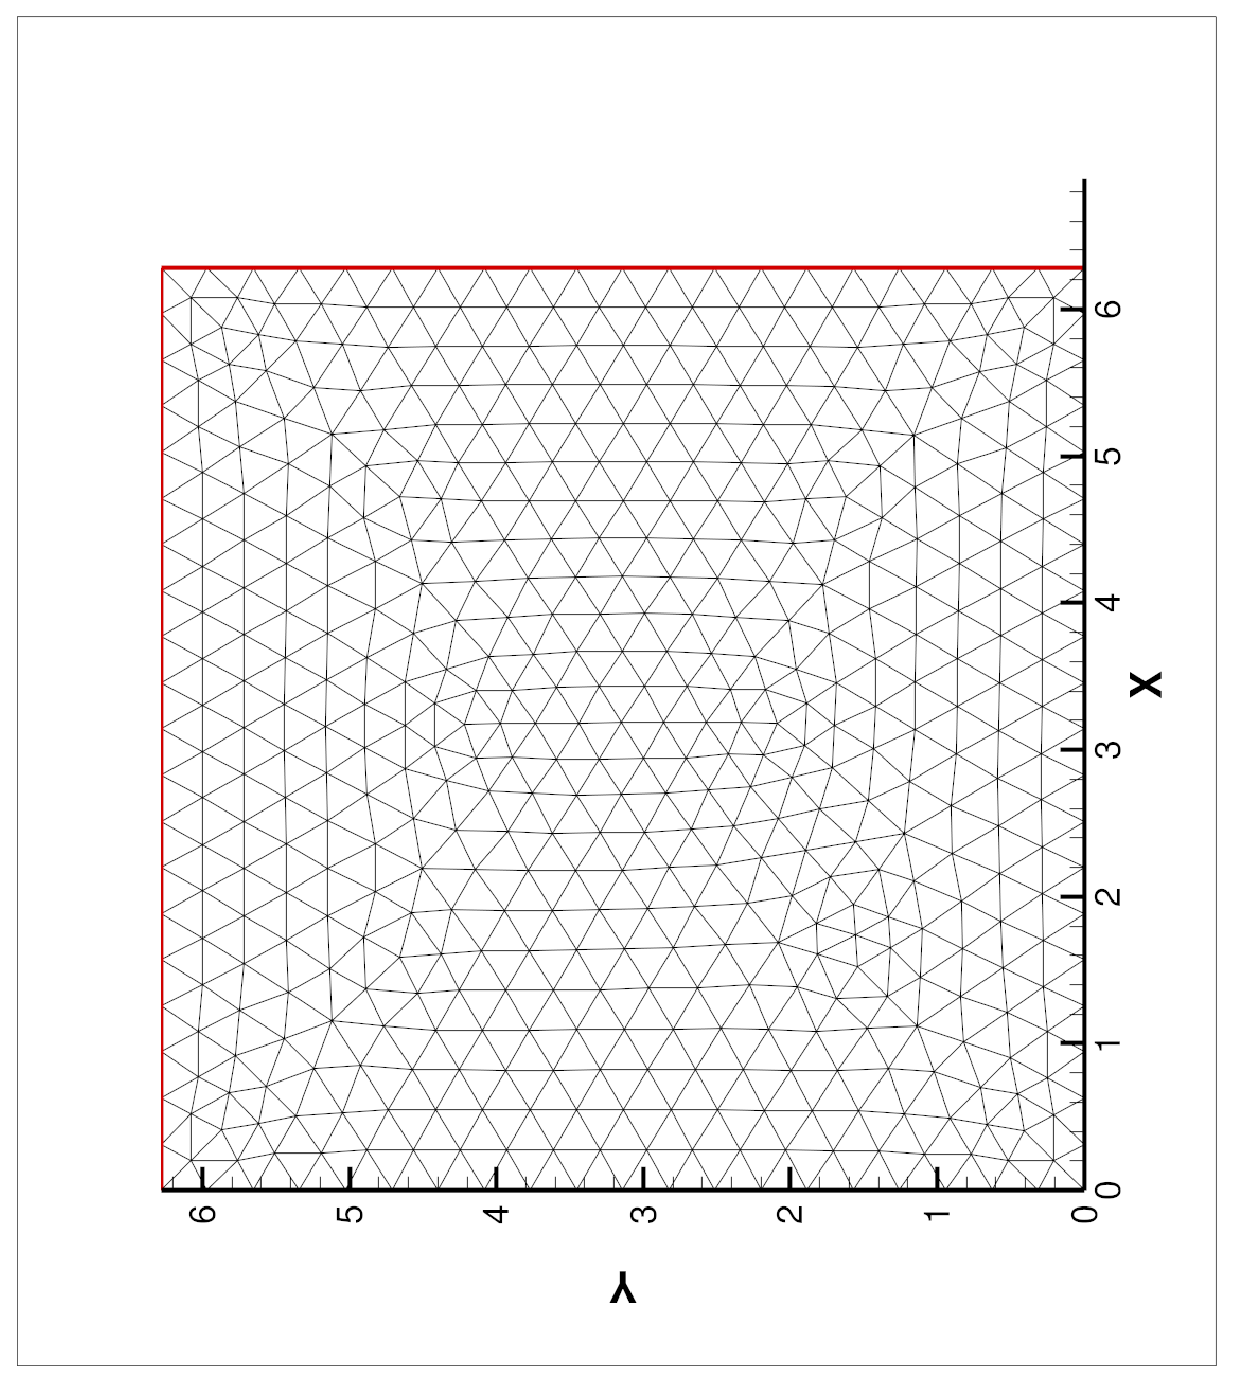
\includegraphics[width = 0.43\textwidth, angle = -90]{./uniform20_meshP.eps}
   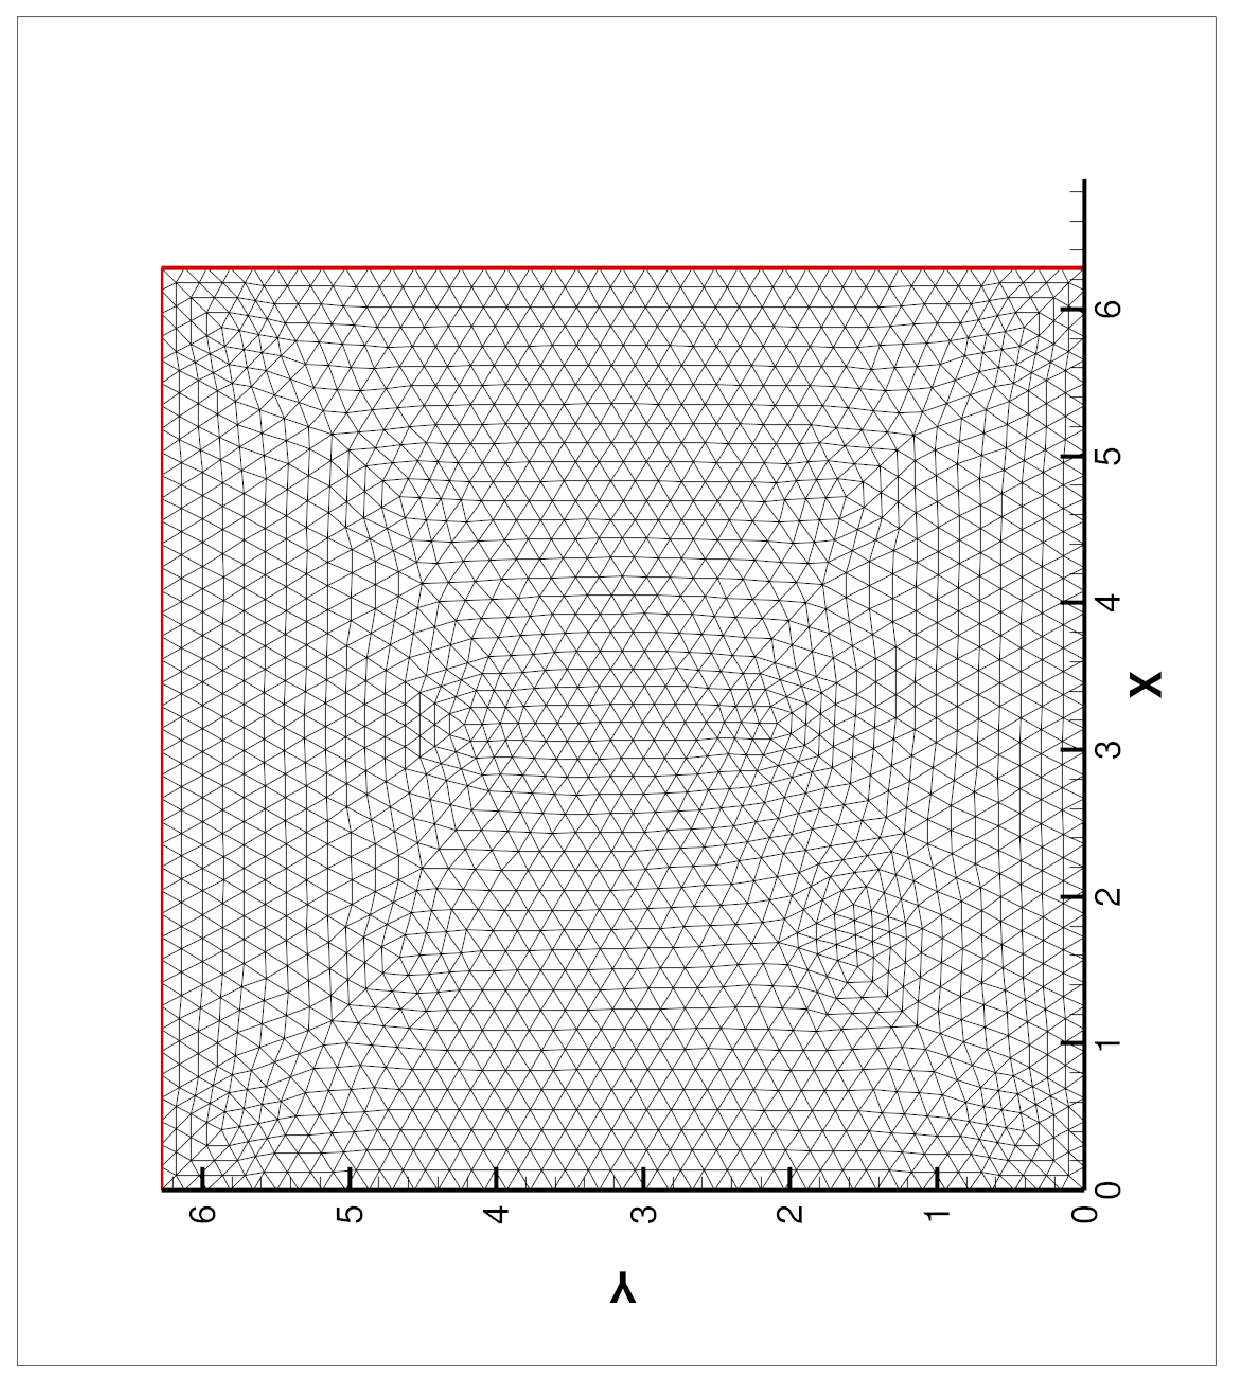
\includegraphics[width = 0.43\textwidth, angle = -90]{./uniform20_meshV.eps}
   \caption{\small Uniform mesh $20 \times 20$,
     Left: mesh P, right: mesh V, $t = 1s, \nu = 0.05$.}
   \label{fig::uniform20_mesh}
 \end{figure}

 \begin{figure}[ht]
   \centering
   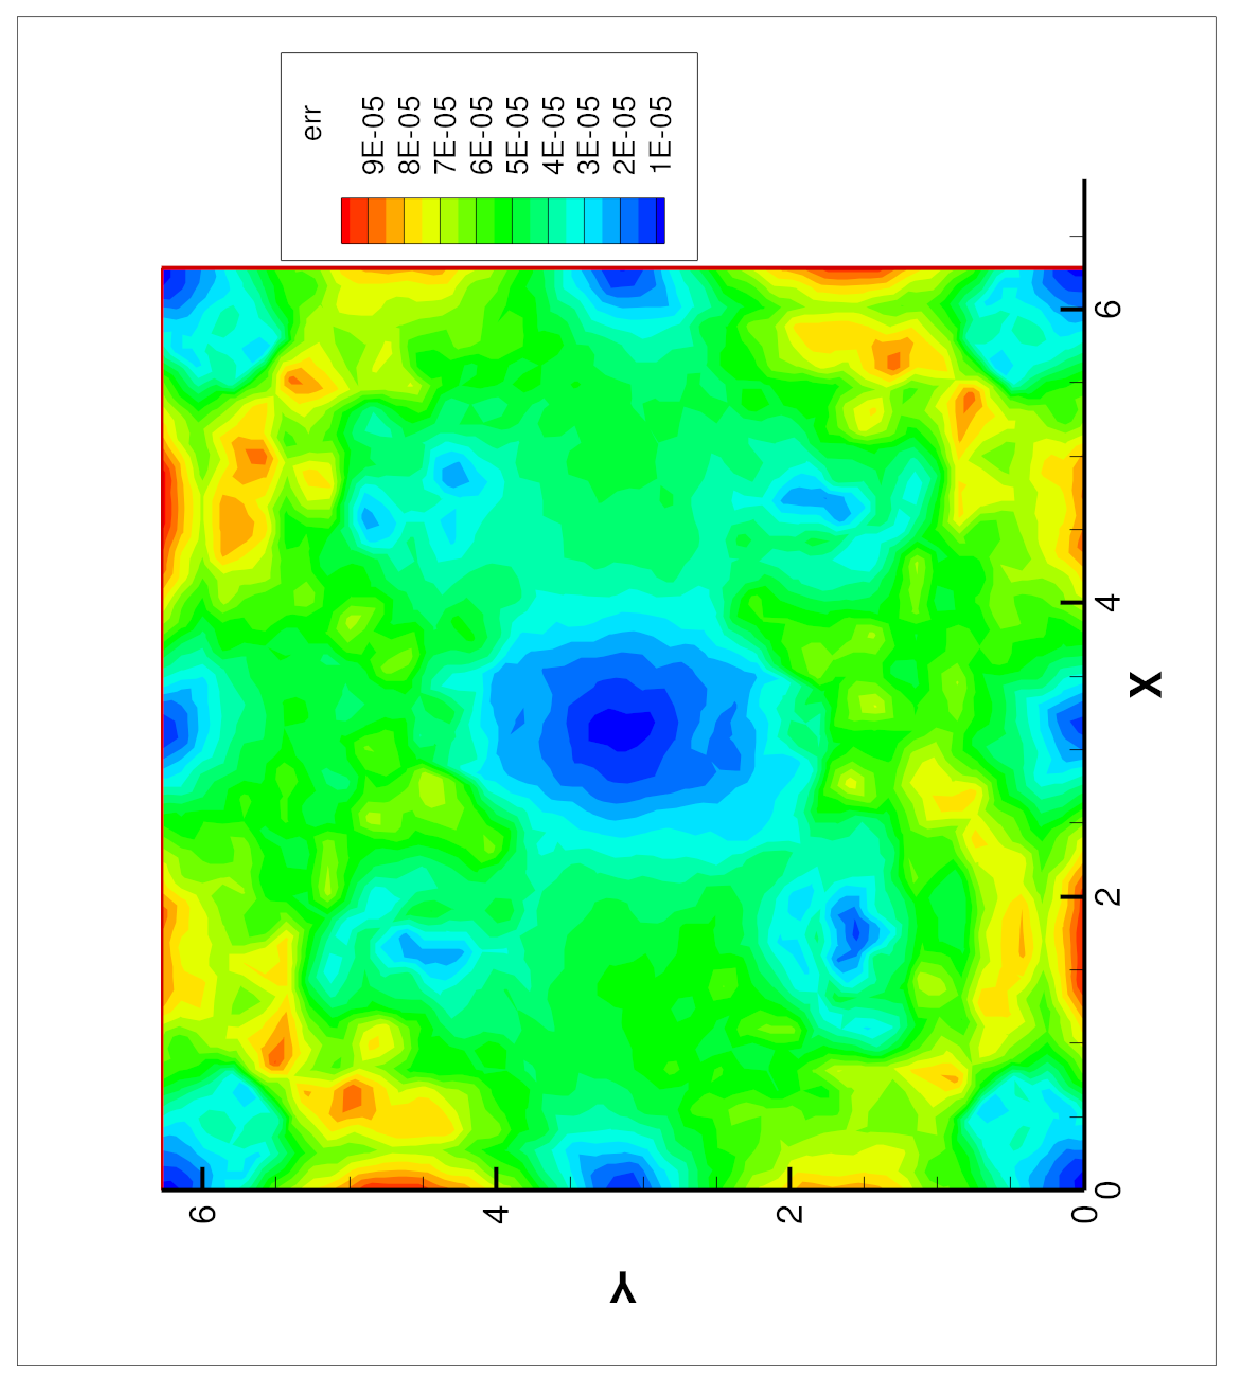
\includegraphics[width = 0.43\textwidth, angle = -90]{./uniform20_error.eps}
   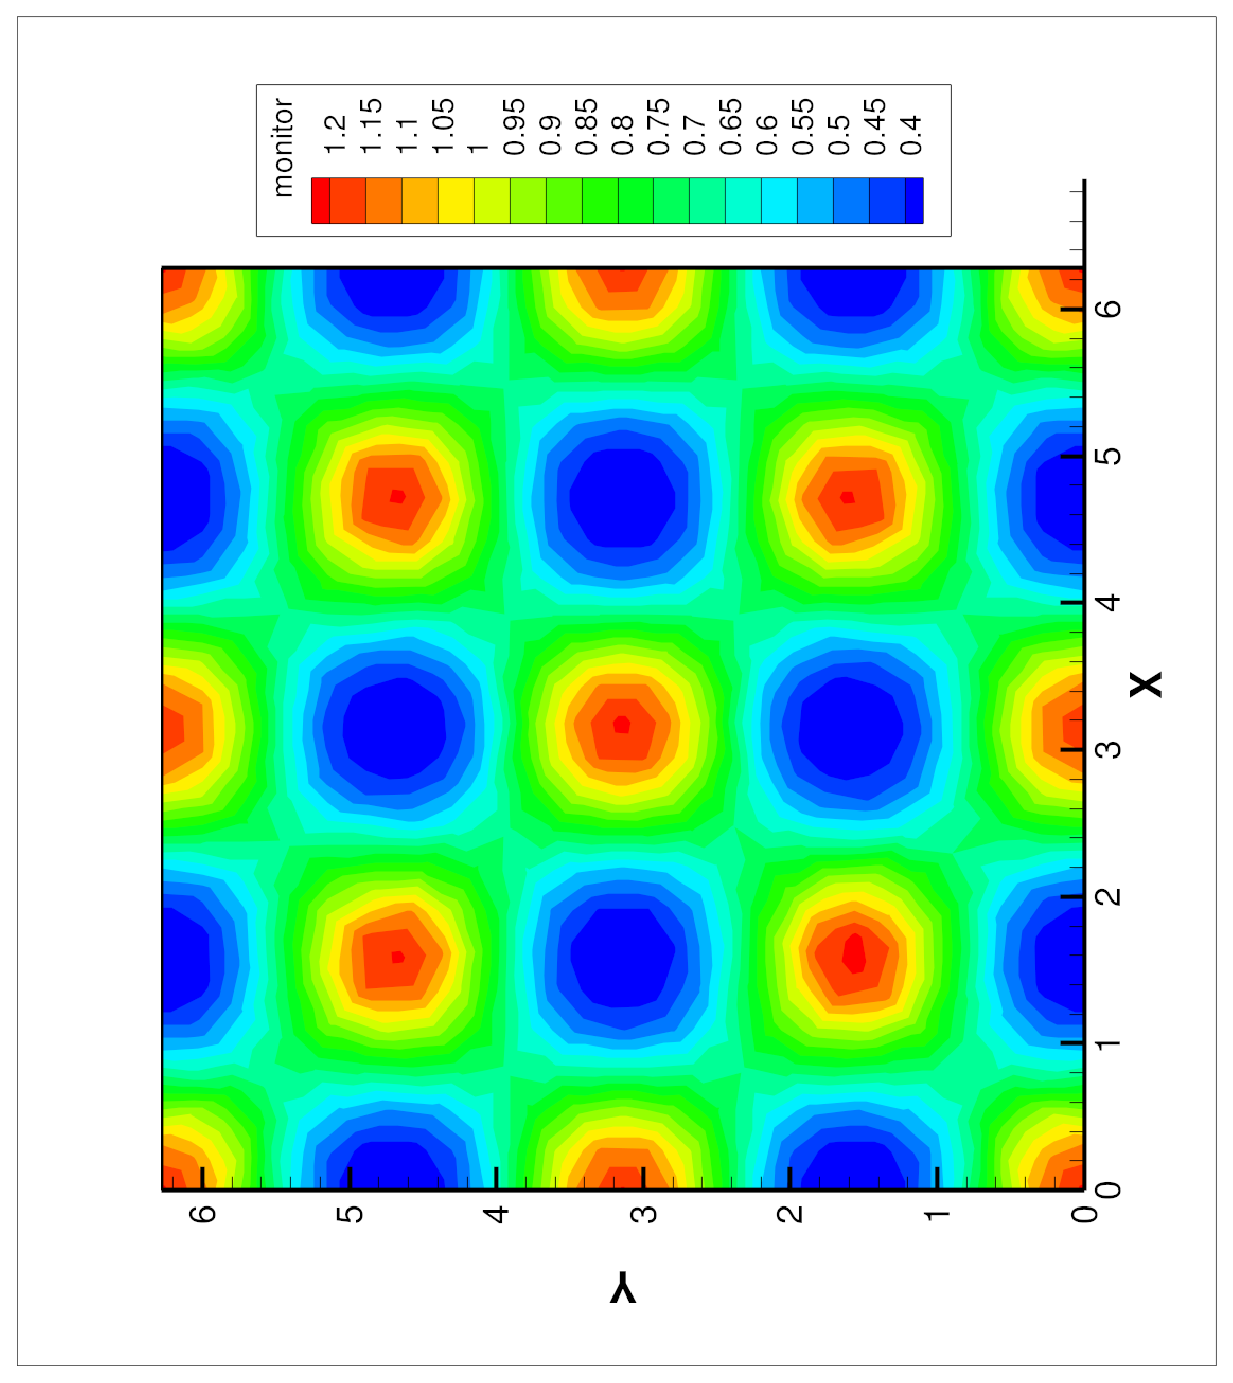
\includegraphics[width = 0.43\textwidth, angle = -90]{./uniform20_monitor.eps}
   \caption{\small Uniform mesh $20 \times 20$ Left: distribution of
     $||\vec{u} - \vec{u}_h||_{L^2}$ error, right: monitor $G_1$ in \ref{eq::monitor_u_h}.}
   \label{fig::uniform20_error_monitor}
 \end{figure}

\subsubsection{Mesh 40 * 40}

 In Figure (\ref{fig::uniform40_solution}), velocity streamline and
 pressure contour is present.

 \begin{figure}[ht]
   \centering
   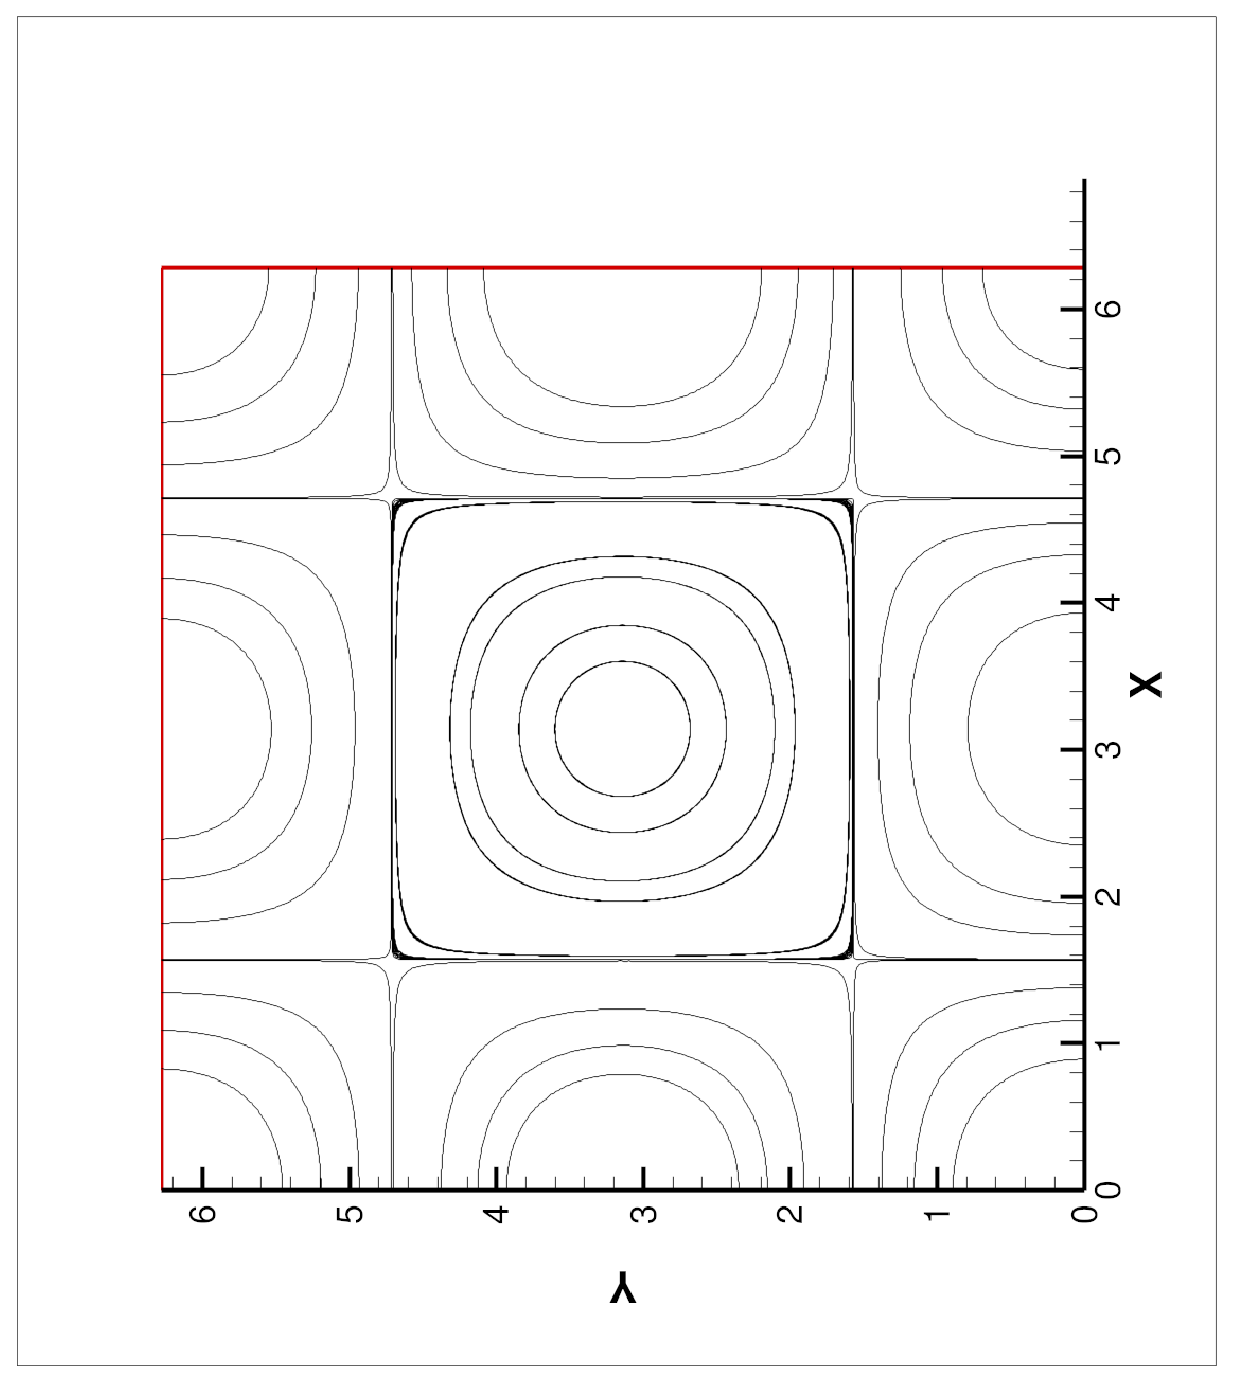
\includegraphics[width = 0.43\textwidth, angle = -90]{./uniform40_streamline.eps}
   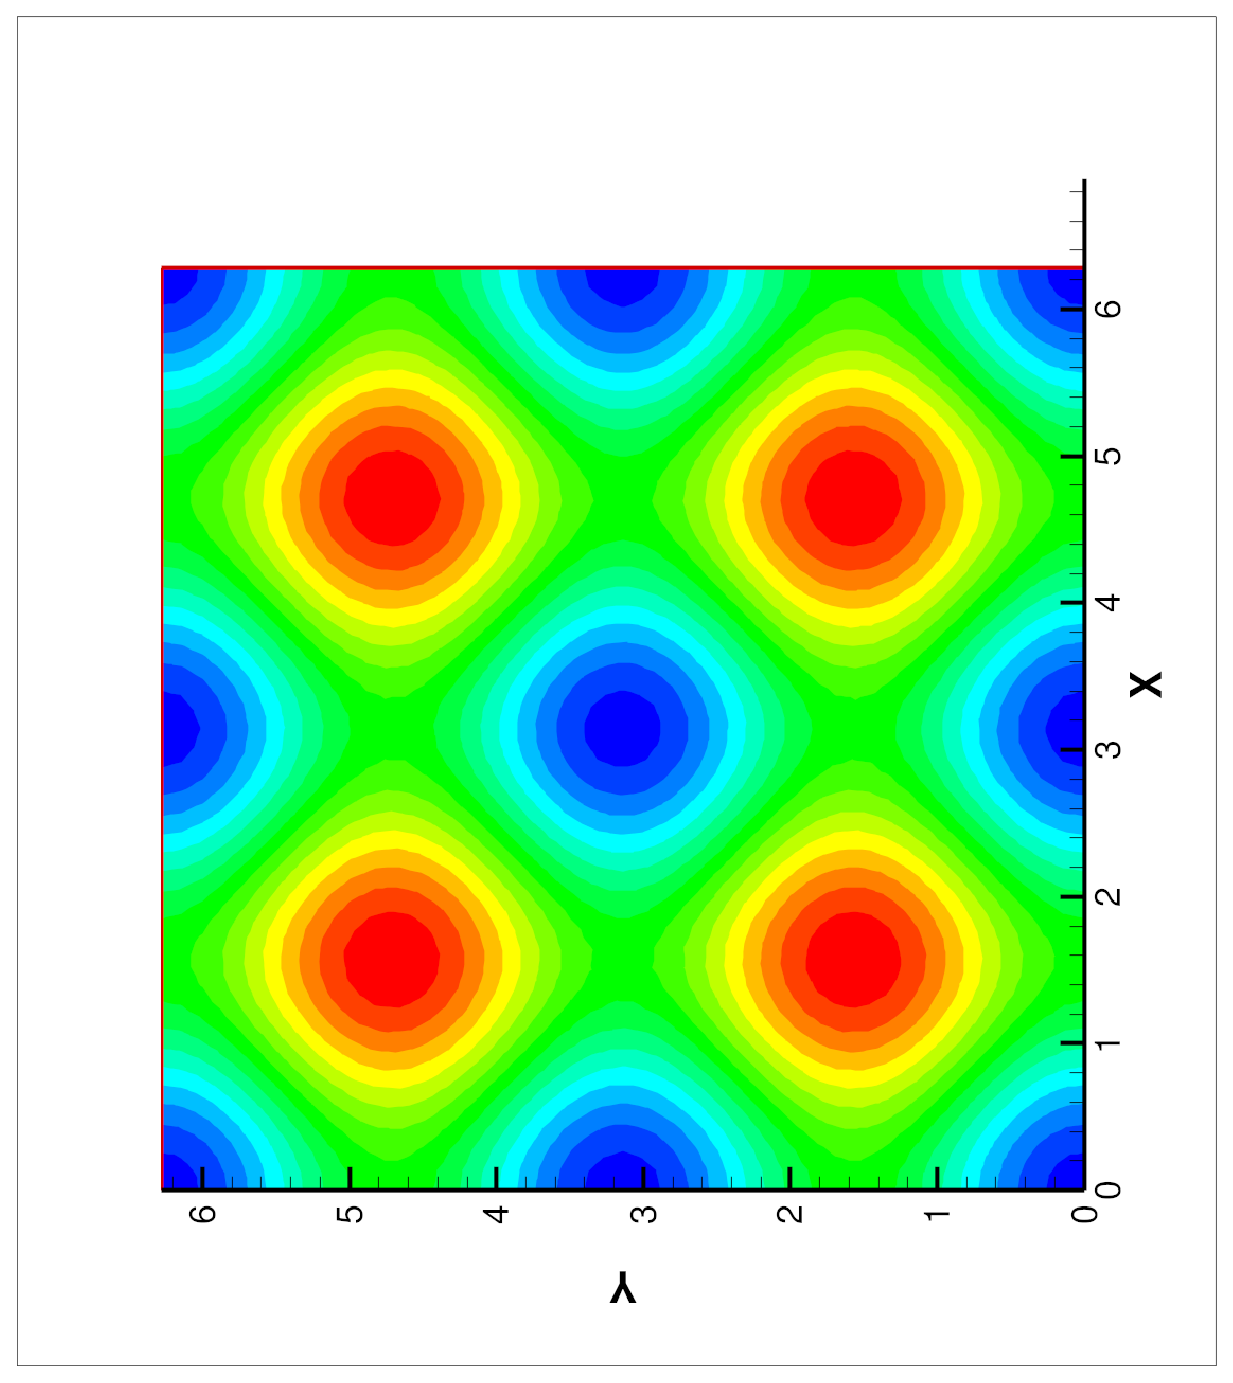
\includegraphics[width = 0.43\textwidth, angle = -90]{./uniform40_pressure.eps}
   \caption{\small Uniform mesh $40 \times
     40$, Left: streamline, right: pressure contour. $t = 1s, \nu = 0.05$.}
   \label{fig::uniform40_solution}
 \end{figure}

 \begin{figure}[ht]
   \centering
   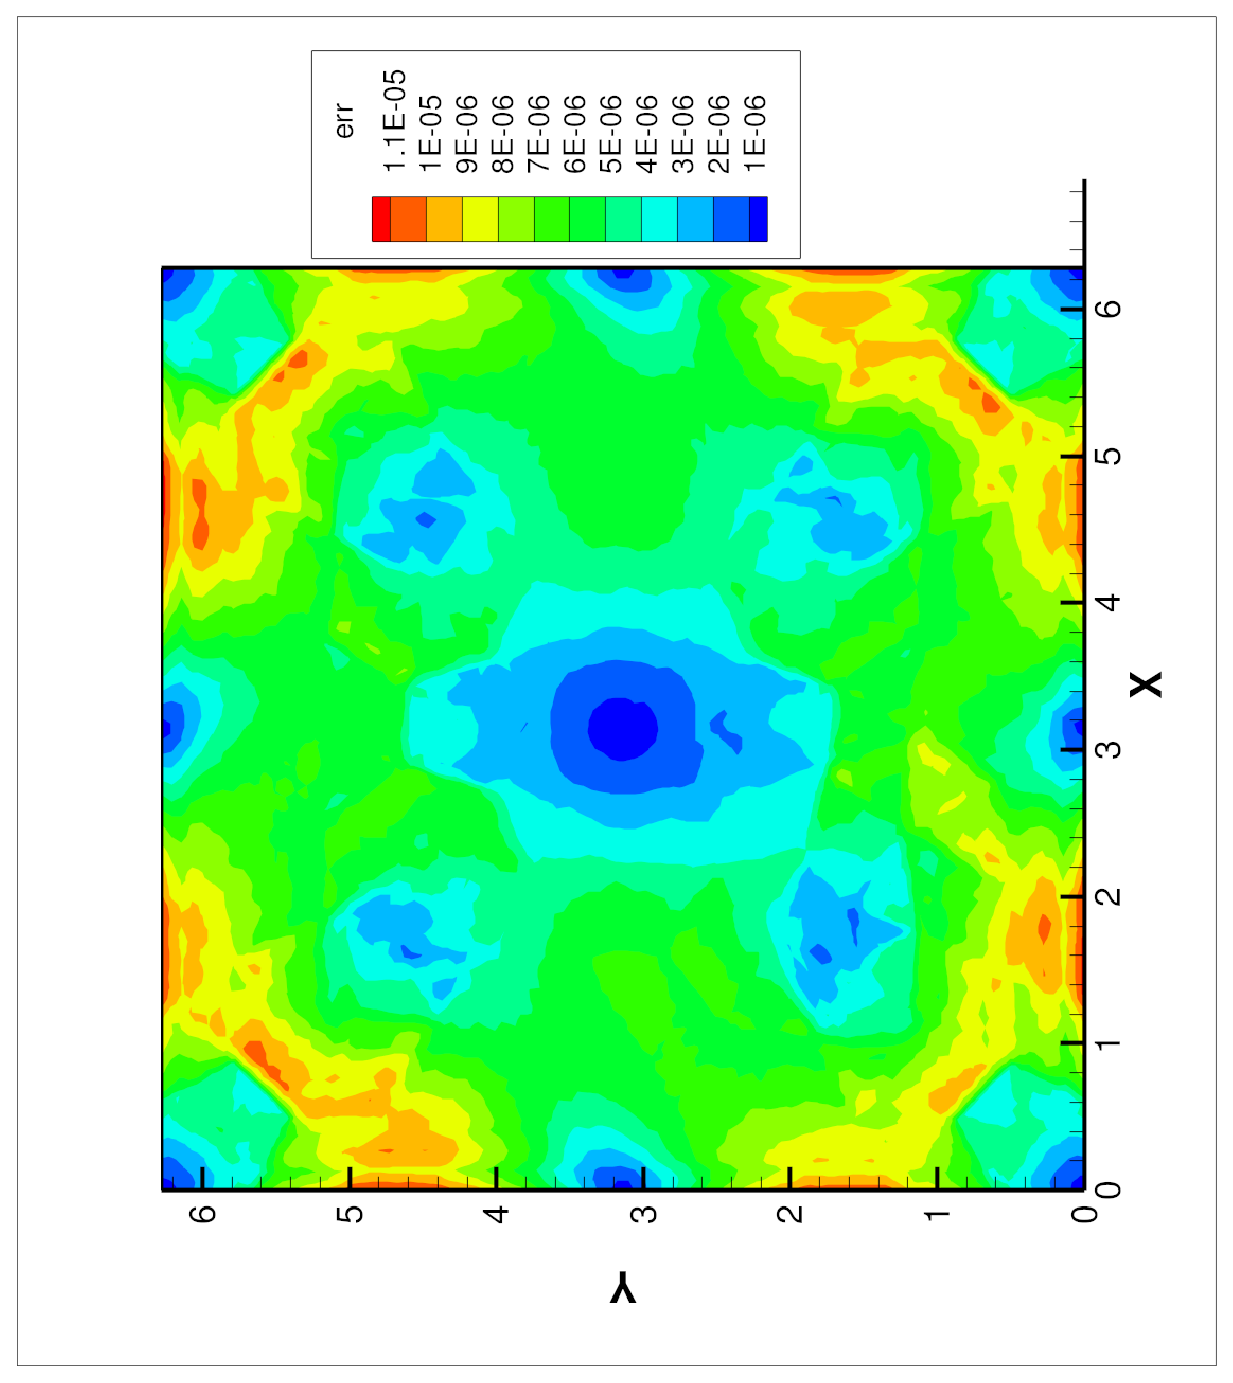
\includegraphics[width = 0.43\textwidth, angle = -90]{./uniform40_error.eps}
   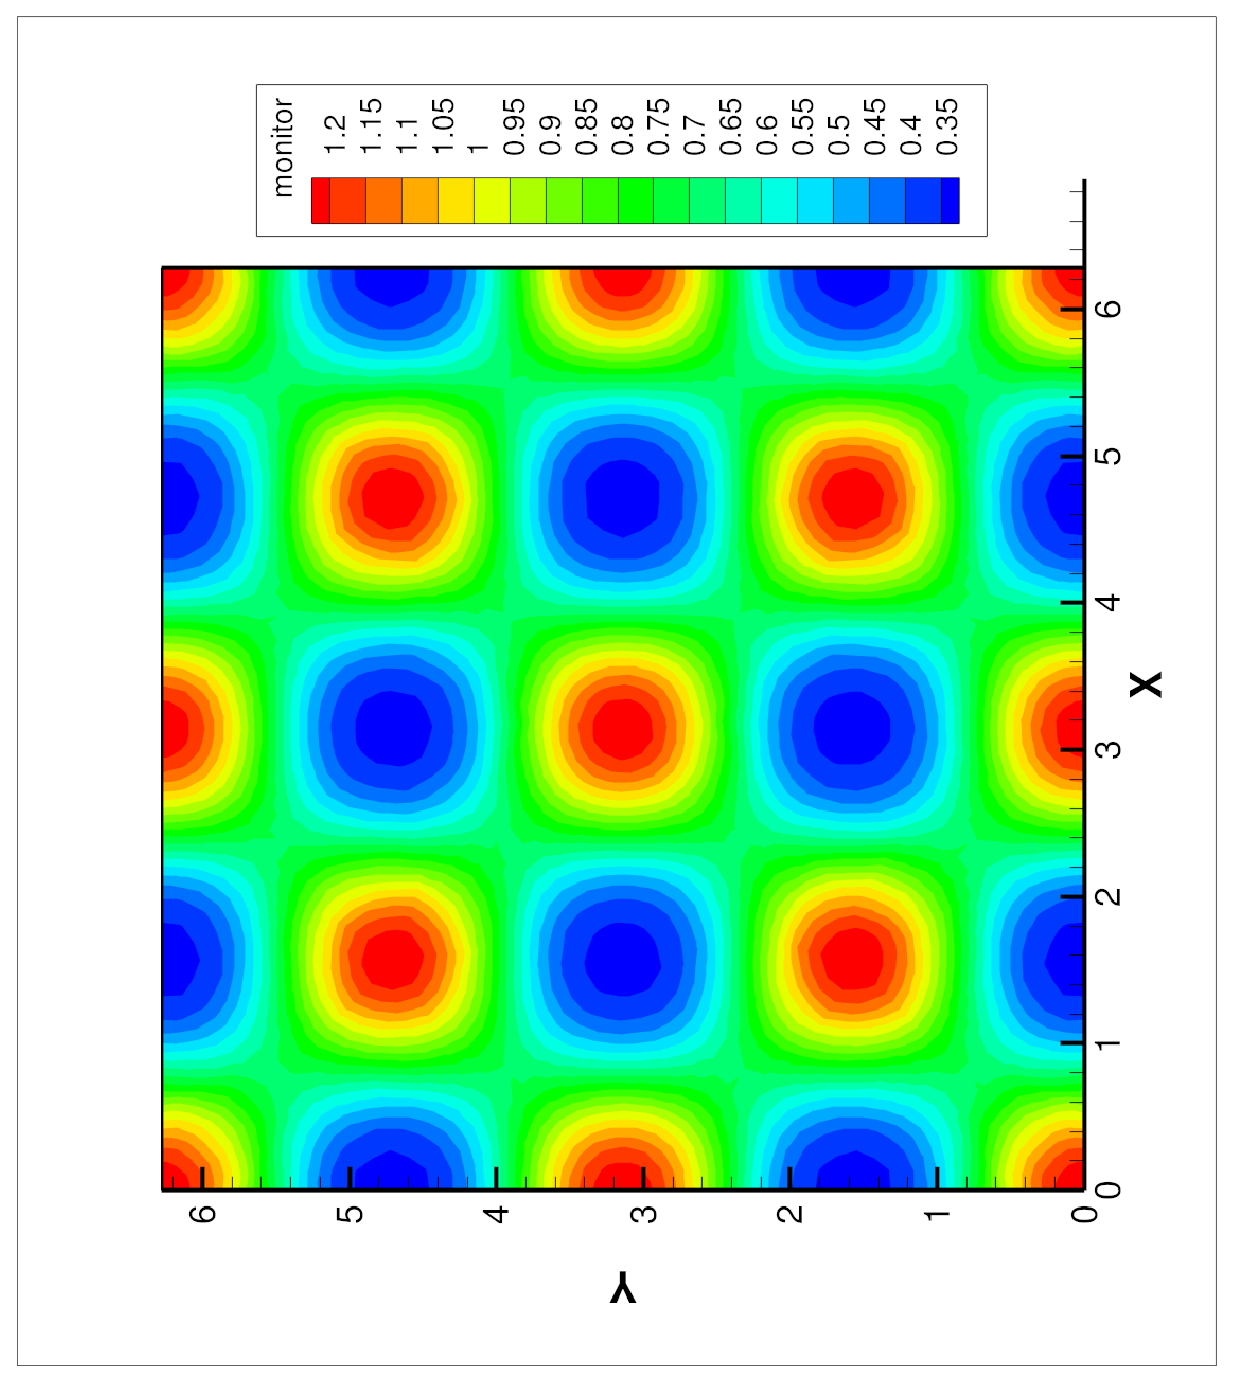
\includegraphics[width = 0.43\textwidth, angle = -90]{./uniform40_monitor.eps}
   \caption{\small Uniform mesh $40 \times 40$ Left: distribution of
     $||\vec{u} - \vec{u}_h||_{L^2}$ error, right: monitor $G_1$ in \ref{eq::monitor_u_h}.}
   \label{fig::uniform40_error_monitor}
 \end{figure}


\subsection{Moving Mesh}
  We choose 
  \begin{equation}
    G_1 = \sqrt{1.0 + \alpha {|\nabla \vec{u}|}^{\beta}}
    \label{eq::monitor_u_h}
  \end{equation}
  as monitor, here $\alpha$ and $\beta$ are two positive constants.
  In follow experiments, we set $\alpha = 5, \beta = 2$.

  \subsubsection{Error analysis}
  
\begin{table}[!htbp]
  \centering
  \begin{tabular}{ccccccc} \toprule
    Mesh (P)  & $||u - u_h ||_{L^2}$ & $||u - u_h ||_{H^1}$ & $||v -
    v_h||_{L^2}$ & $||v - v_h||_{H^1}$ & $||p - p_h||_{L^2}$ & $||p -
    p_h||_{H^1}$ \\ \midrule
    $20 \times 20$ &   $1.113 e{-2}$    & $2.960 e{-1}$ &
    $1.124 e{-2}$   &$2.961 e{-1}$   &   $4.117 
    e{-2}$ &   $4.666  e{-1}$ \\ \midrule
    $40 \times 40$   &   $2.713 e{-3}$   &   $1.517 e{-1}$  &
    $2.693   e{-3}$ & $1.511   e{-1}$ &
    $1.613   e{-2}$ & $2.432   e{-1}$ \\ \bottomrule
  \end{tabular}
  \caption{\small Error for Accuracy test using moving mesh, $\nu = 0.05, t = 1s$.}
  \label{tab::accuracy_moving_error}
\end{table}
  
  \subsubsection{Mesh 20 * 20}

 Numerical solution and moving mesh are show in
 FIgure(\ref{fig::moving20_solution}) and Figure(\ref{fig::moving20_mesh}).

 \begin{figure}[ht]
   \centering
   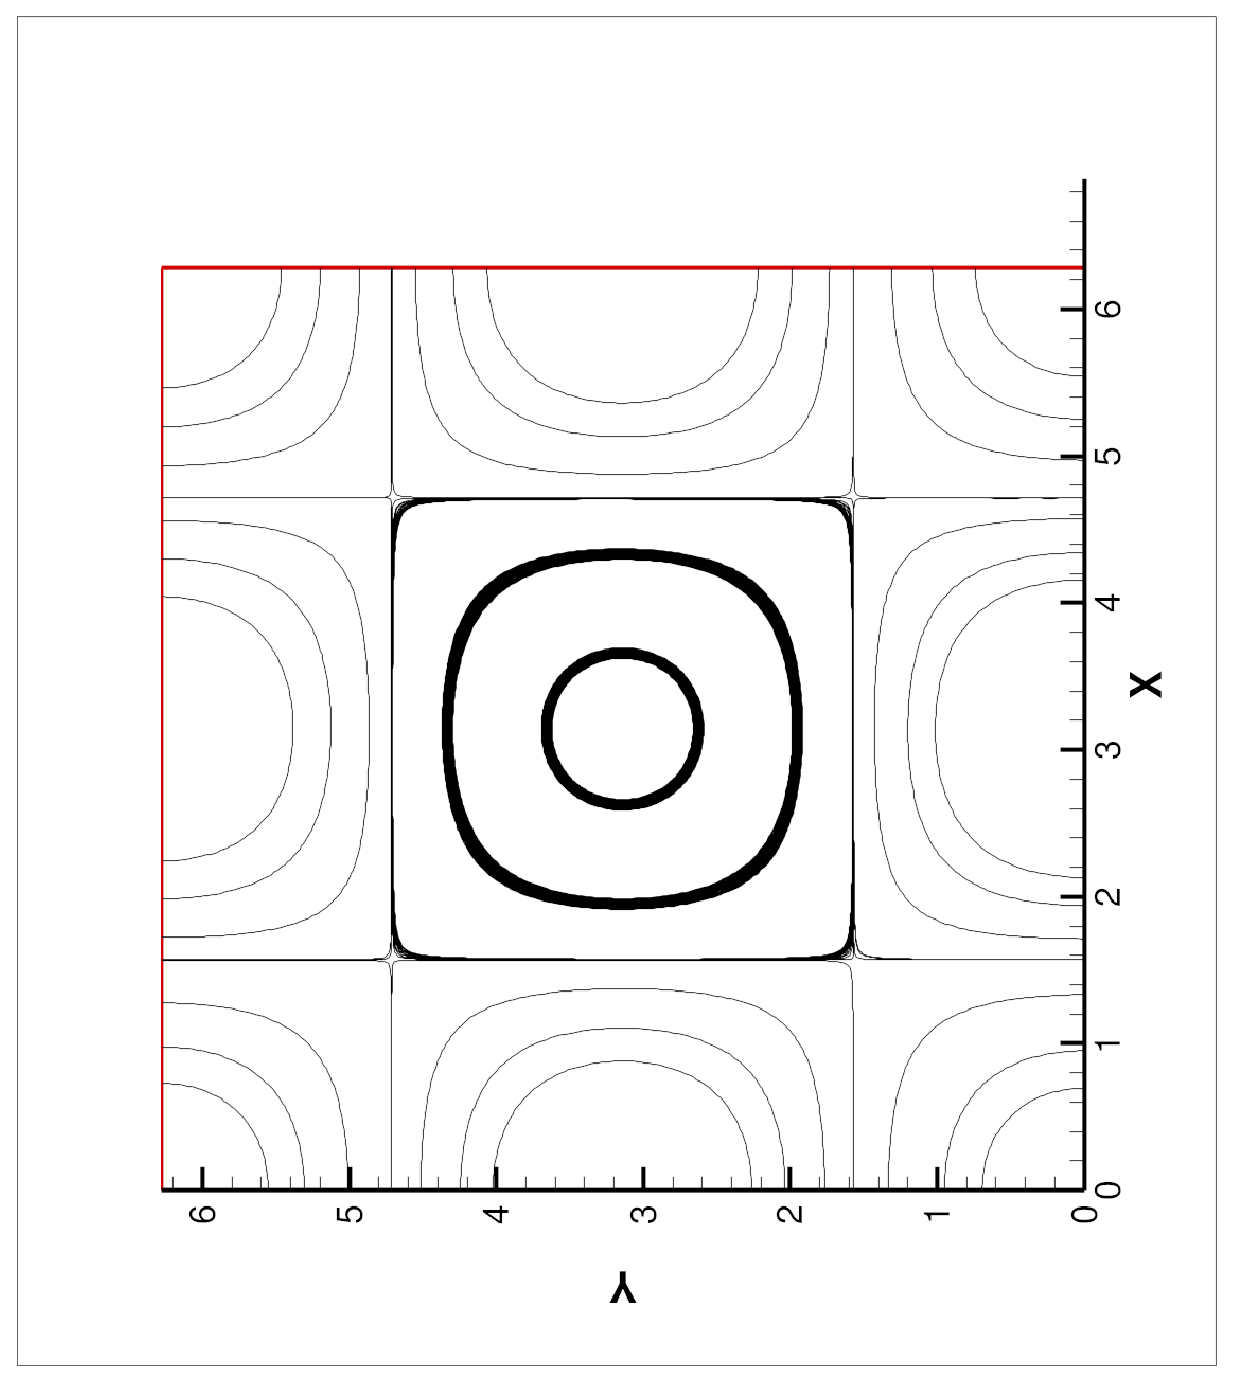
\includegraphics[width = 0.43\textwidth, angle = -90]{./moving20_streamline.eps}
   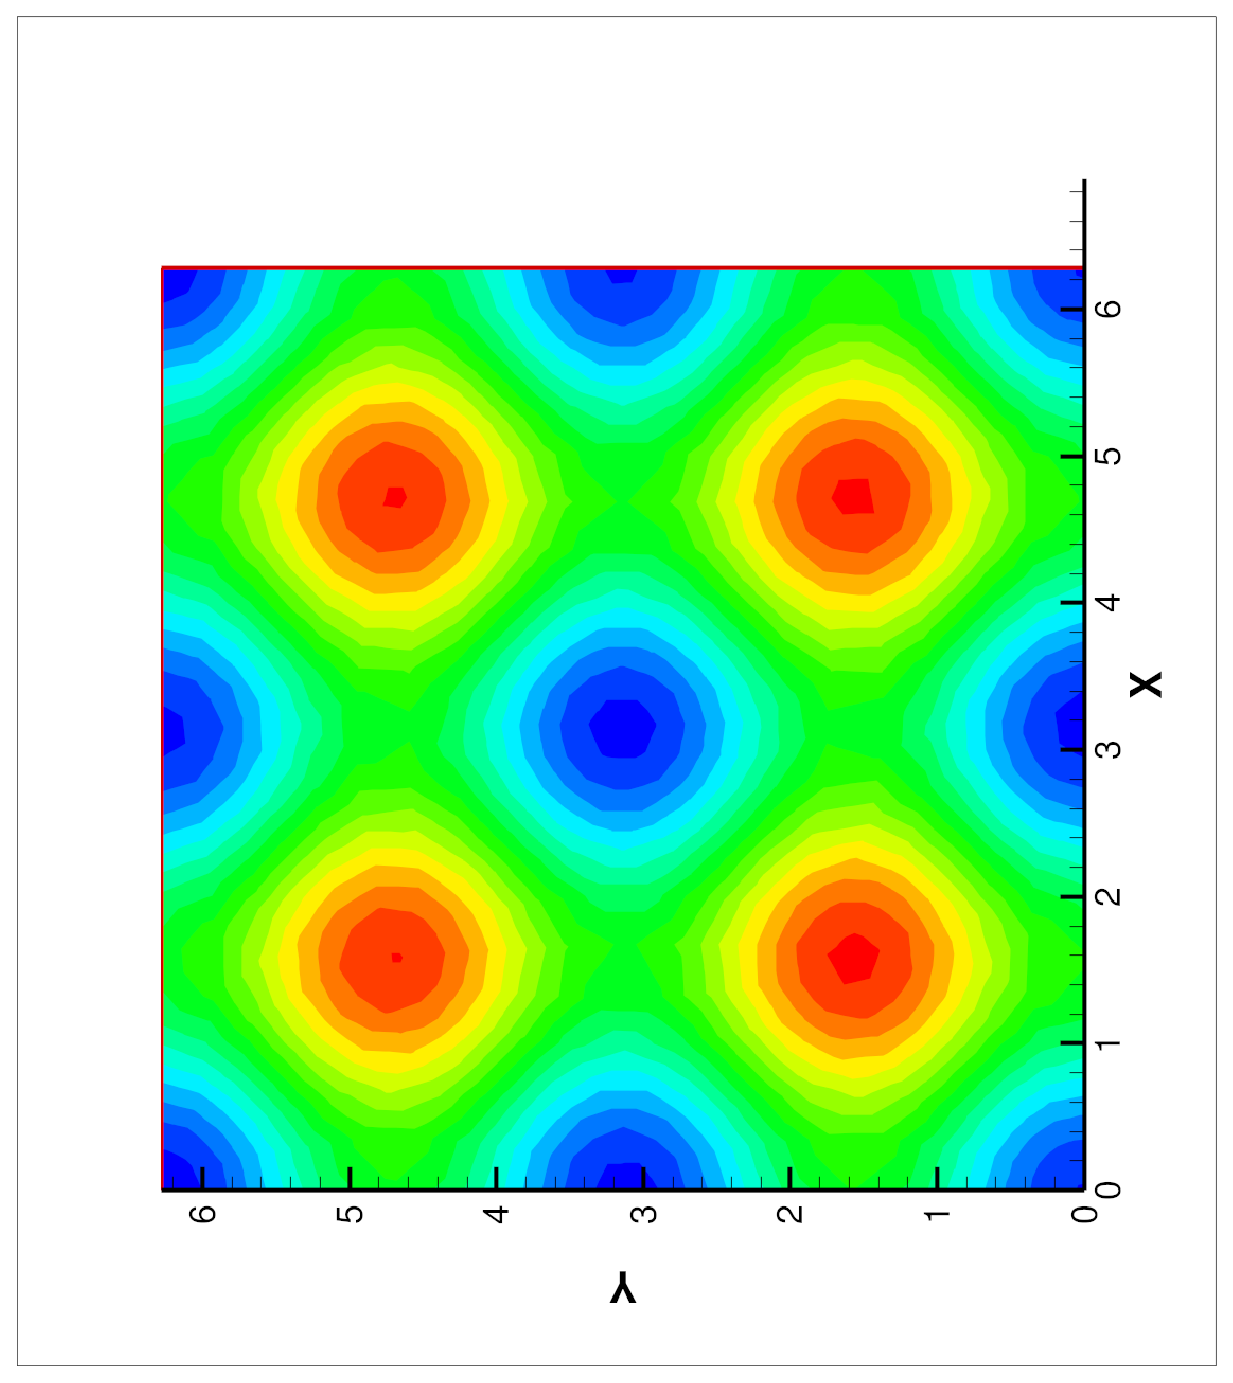
\includegraphics[width = 0.43\textwidth, angle = -90]{./moving20_pressure.eps}
   \caption{\small Moving mesh $20 \times 20$, Left: streamline, right: pressure
     contour. $t = 1s, \nu = 0.05$.}
   \label{fig::moving20_solution}
 \end{figure}

 \begin{figure}[ht]
   \centering
   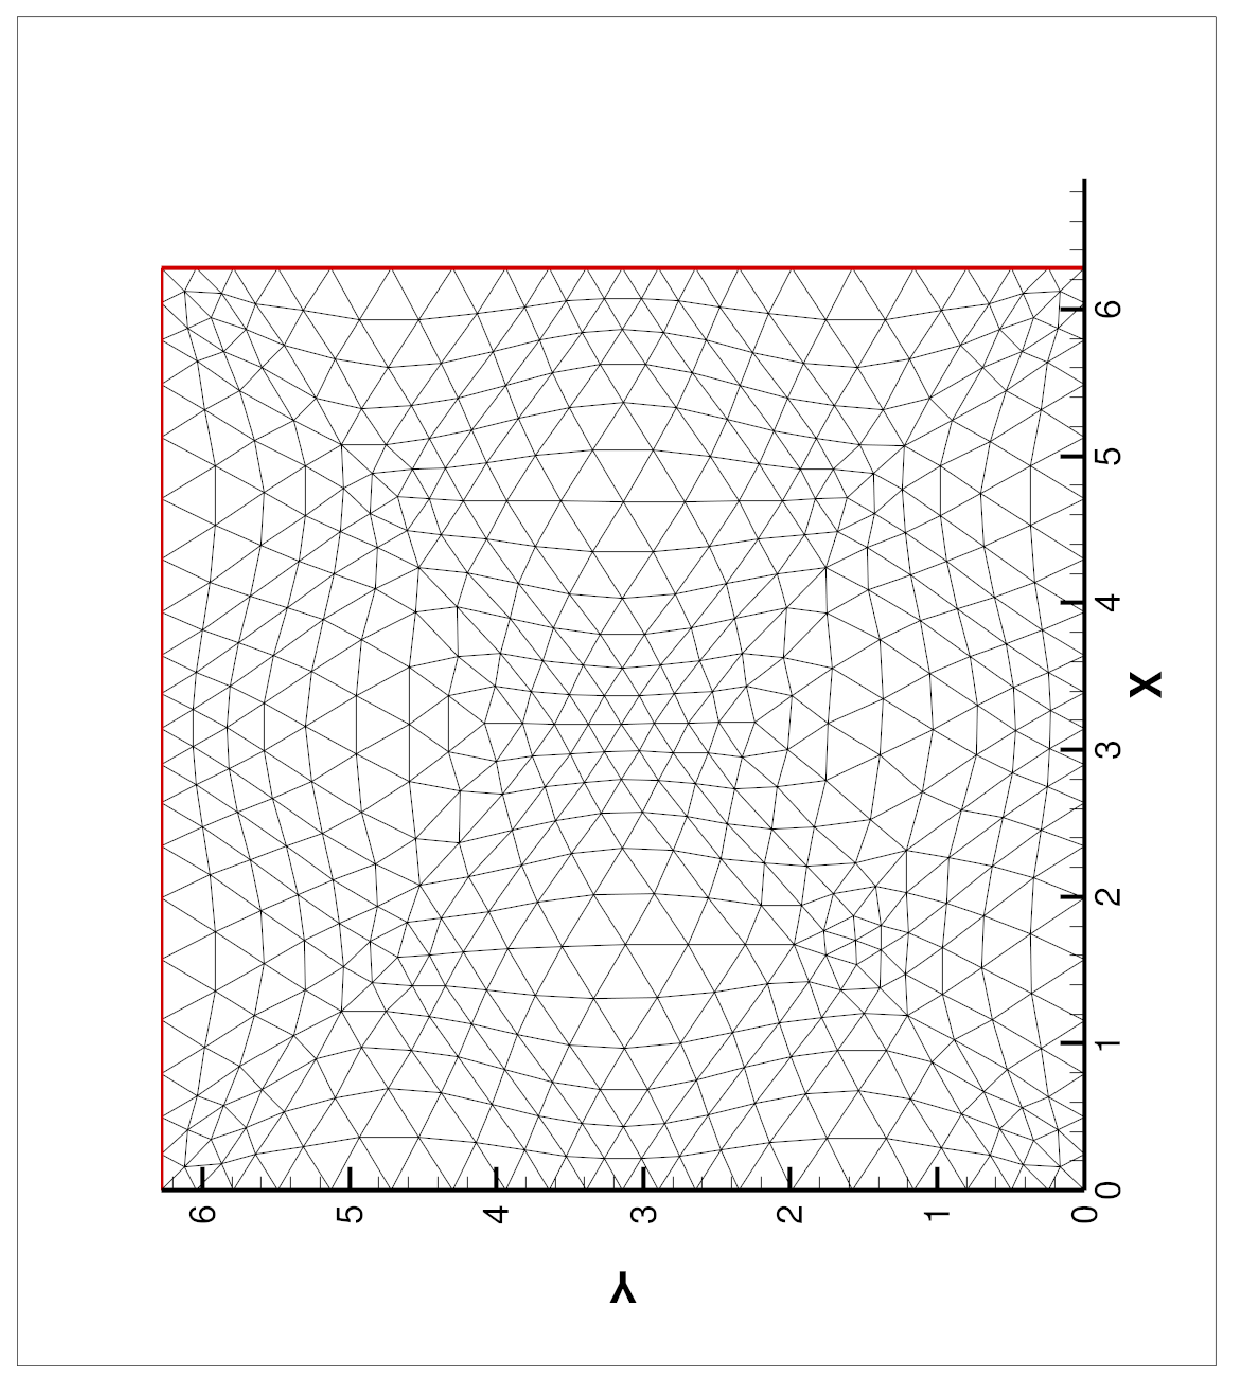
\includegraphics[width = 0.43\textwidth, angle = -90]{./moving20_meshP.eps}
   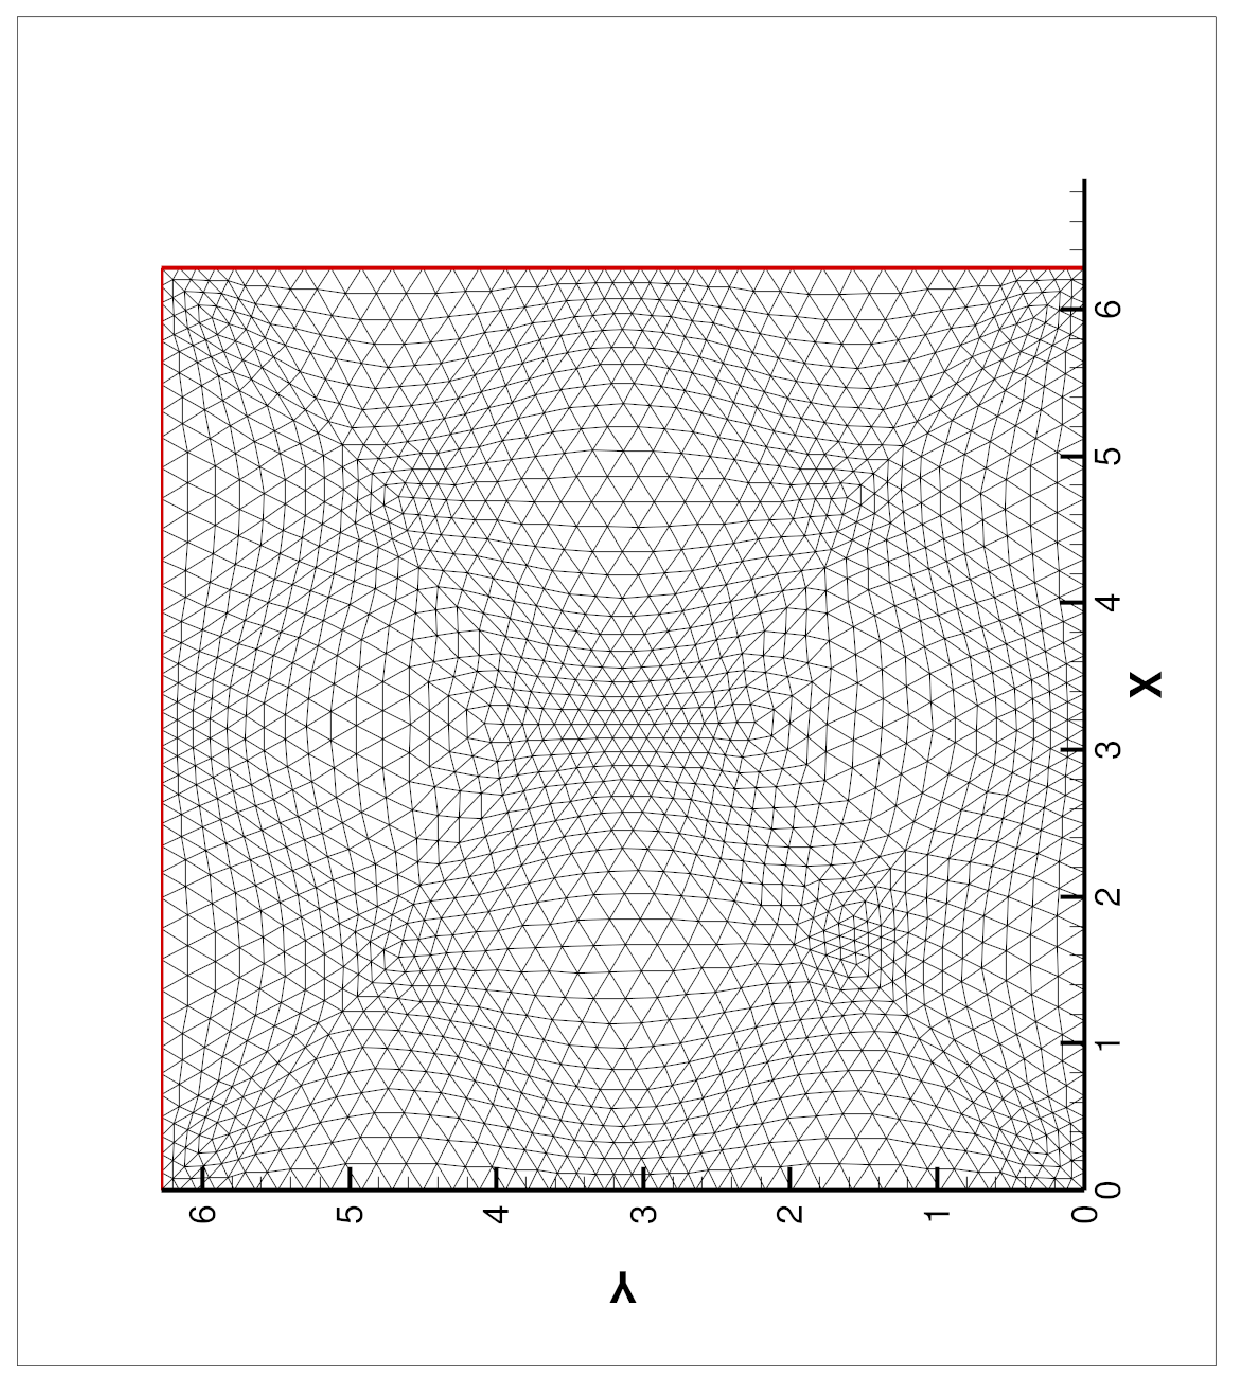
\includegraphics[width = 0.43\textwidth, angle = -90]{./moving20_meshV.eps}
   \caption{\small Moving mesh $20 \times 20$,
     Left: mesh P, right: mesh V, using monitor $G_1$
     in (\ref{eq::monitor_u_h}). $t = 1s, \nu = 0.05$.}
   \label{fig::moving20_mesh}
 \end{figure}

 From Figure(\ref{fig::moving20_monitor}), mesh is moving from the
 place where value of monitor is big to that which value is small.
 
 \begin{figure}[ht]
   \centering
   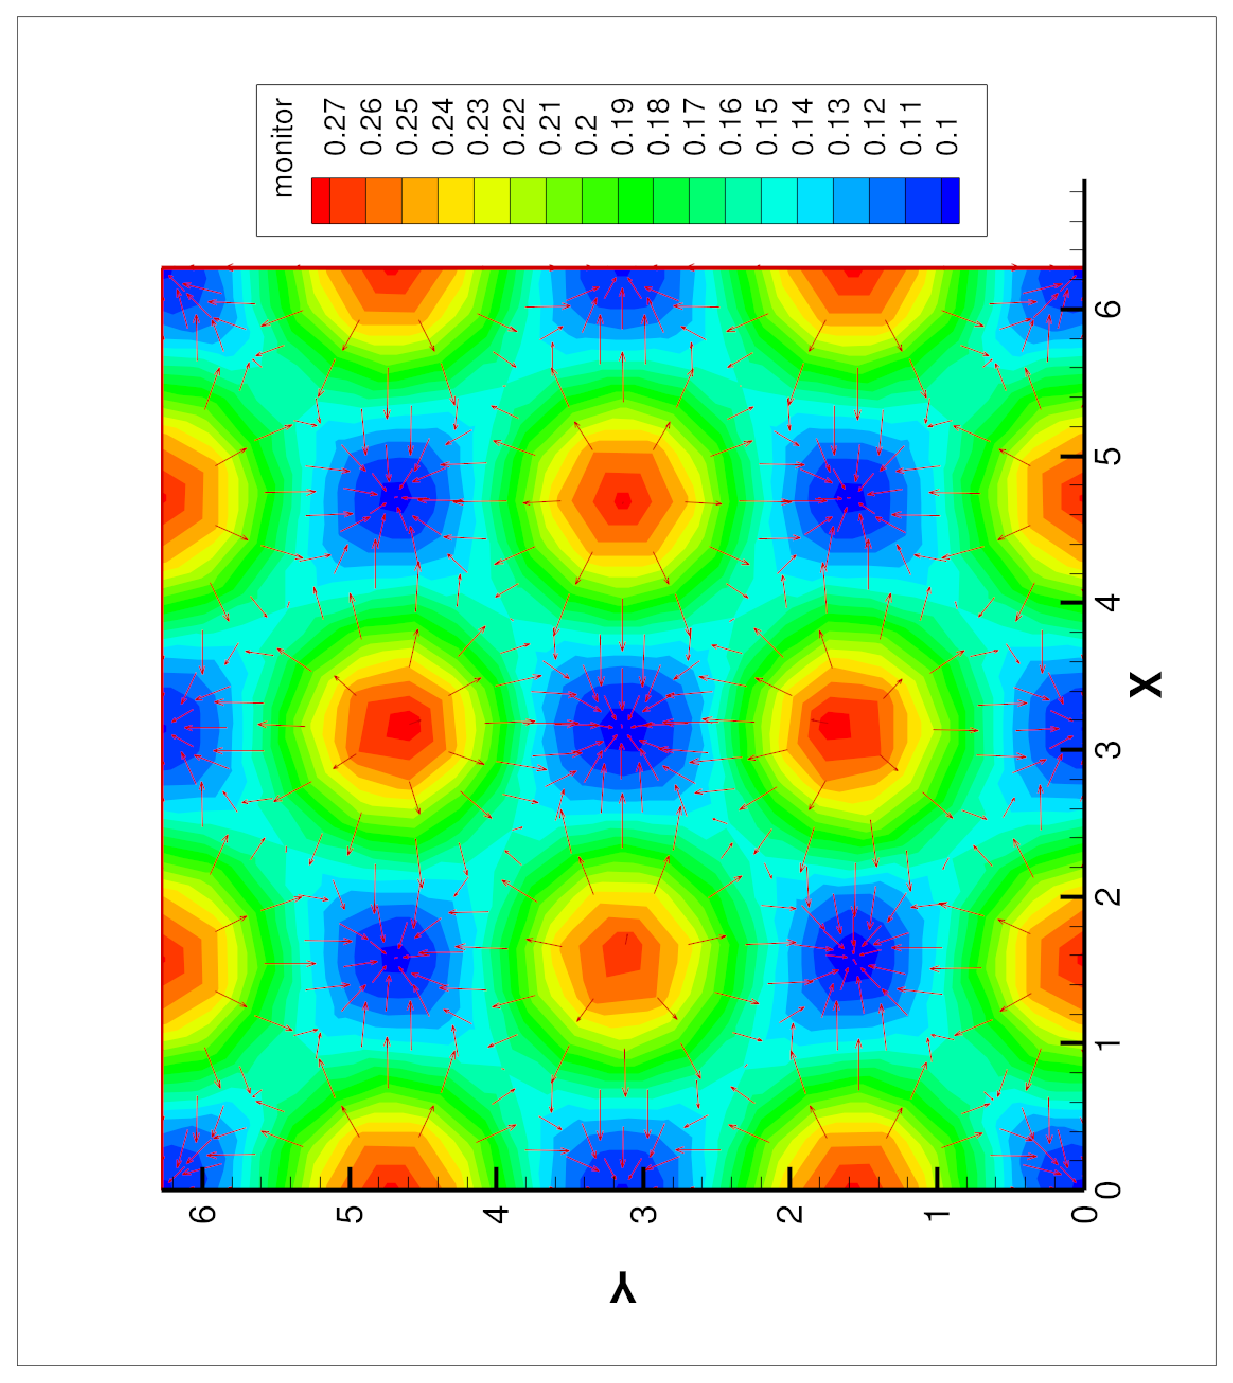
\includegraphics[width = 1.0\textwidth, angle = -90]{./moving20_movedirection.eps}
   \caption{\small Moving mesh $20 \times 20$,
     contour of monitor $m = \frac{1}{G_1}$ in (\ref{eq::monitor_u_h})
     and mesh move direction. $t = 1s, \nu = 0.05$.}
   \label{fig::moving20_monitor}
 \end{figure}

\subsubsection{Mesh 40 * 40}

 \begin{figure}[ht]
   \centering
   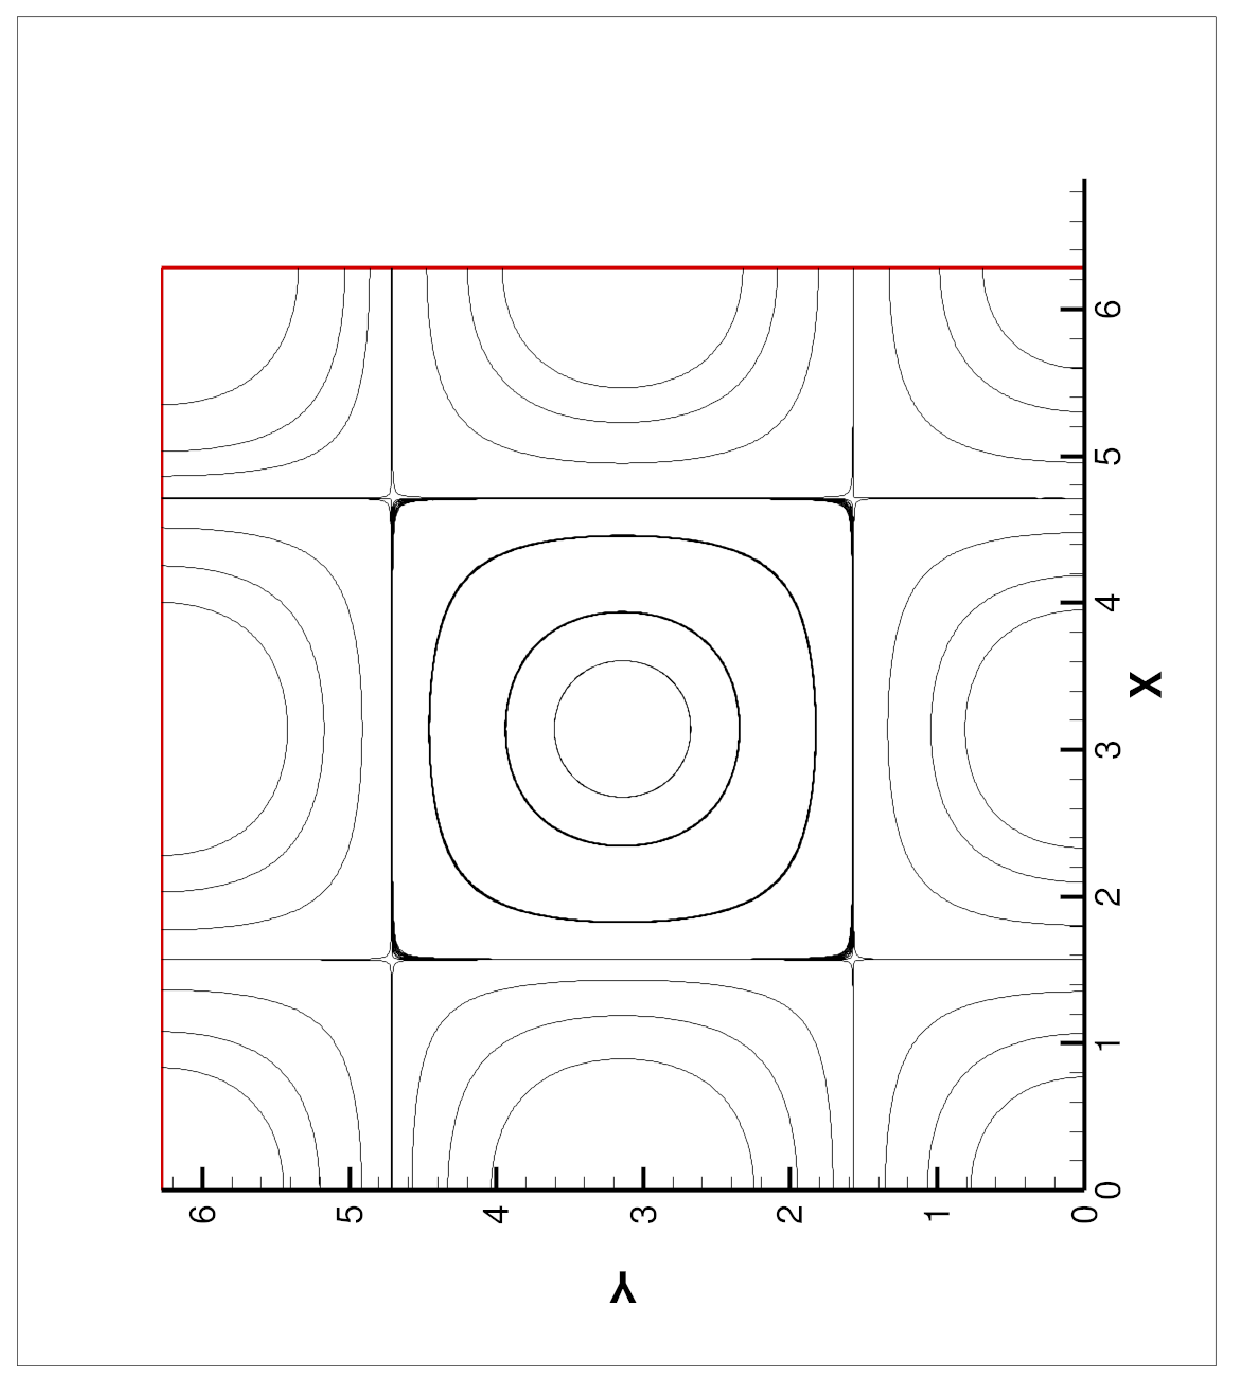
\includegraphics[width = 0.43\textwidth, angle = -90]{./moving40_streamline.eps}
   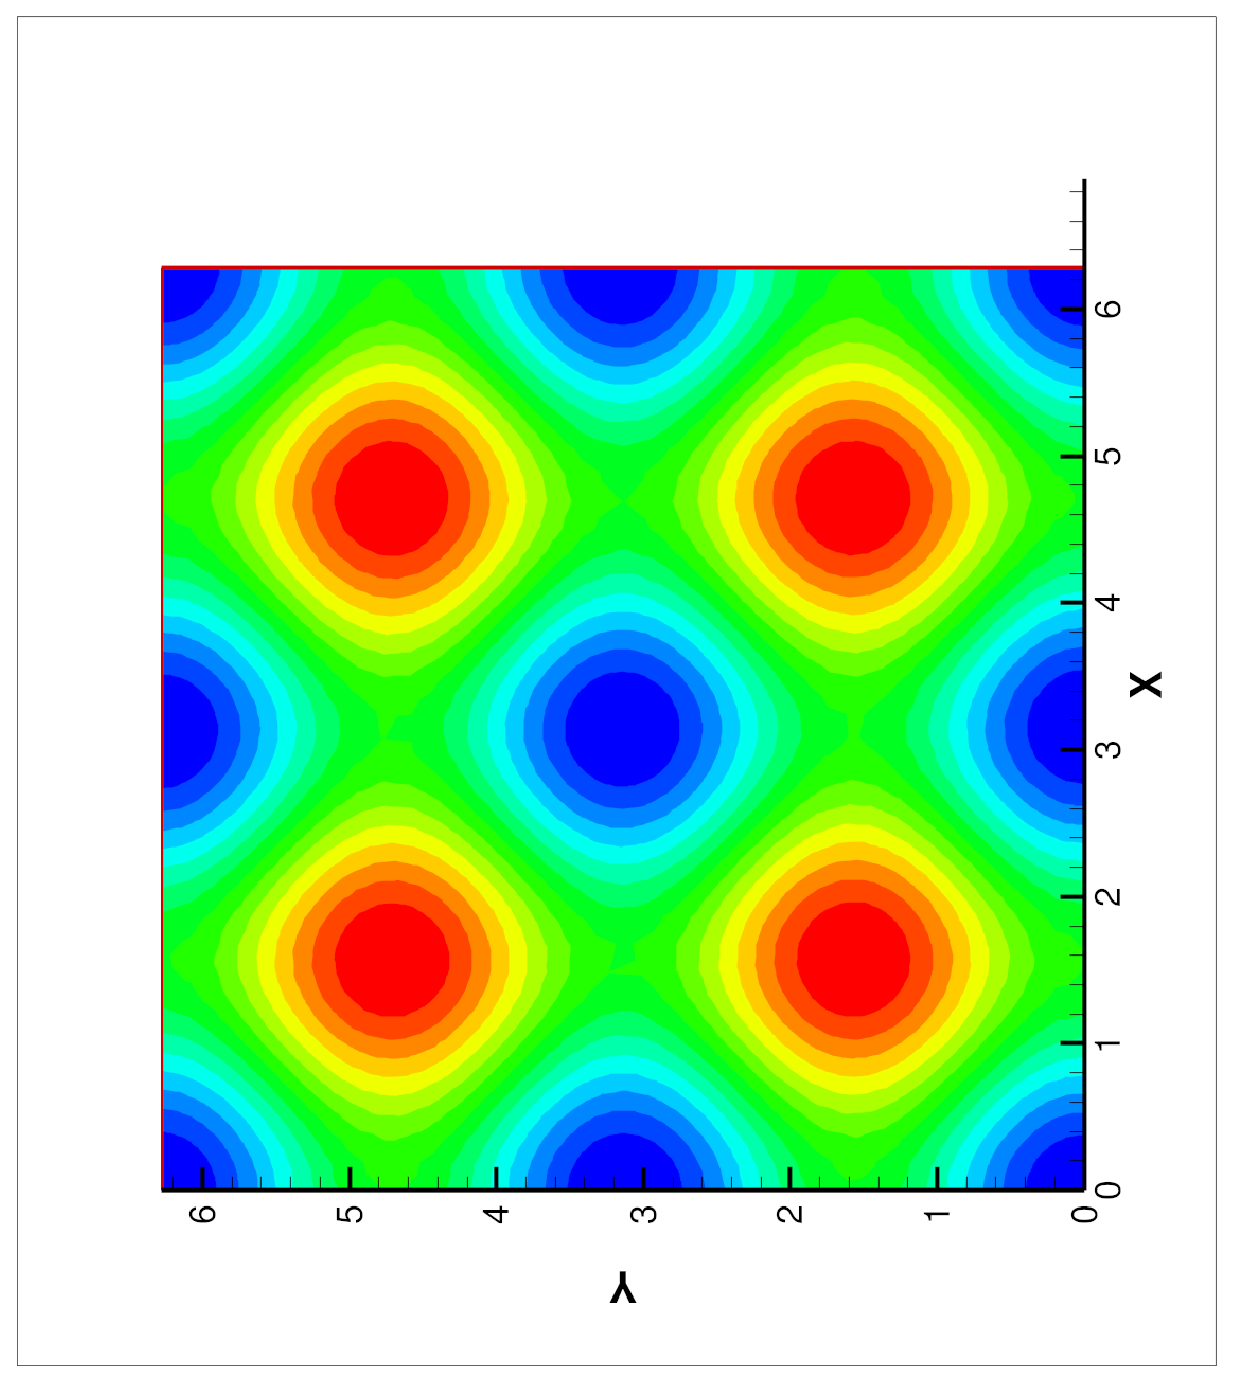
\includegraphics[width = 0.43\textwidth, angle = -90]{./moving40_pressure.eps}
   \caption{\small Moving mesh $40 \times 40$, Left: streamline, right: pressure
     contour. $t = 1s, \nu = 0.05$.}
   \label{fig::moving40_solution}
 \end{figure}

 \begin{figure}[ht]
   \centering
   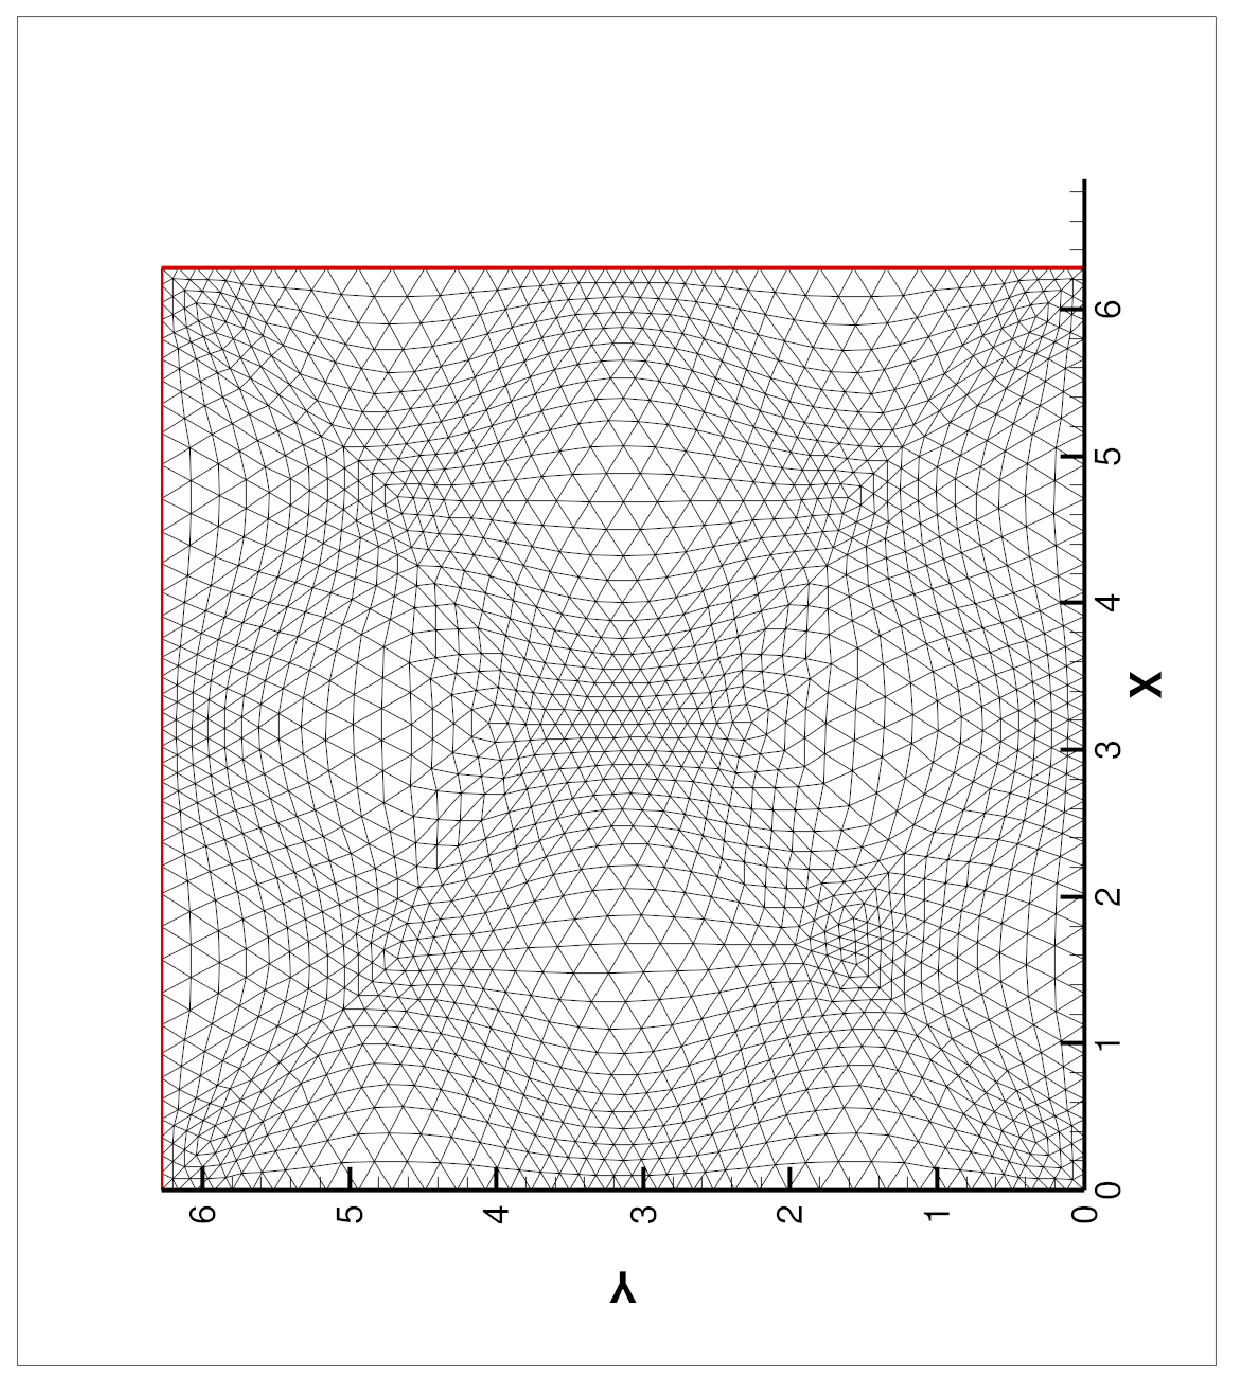
\includegraphics[width = 0.43\textwidth, angle = -90]{./moving40_meshP.eps}
   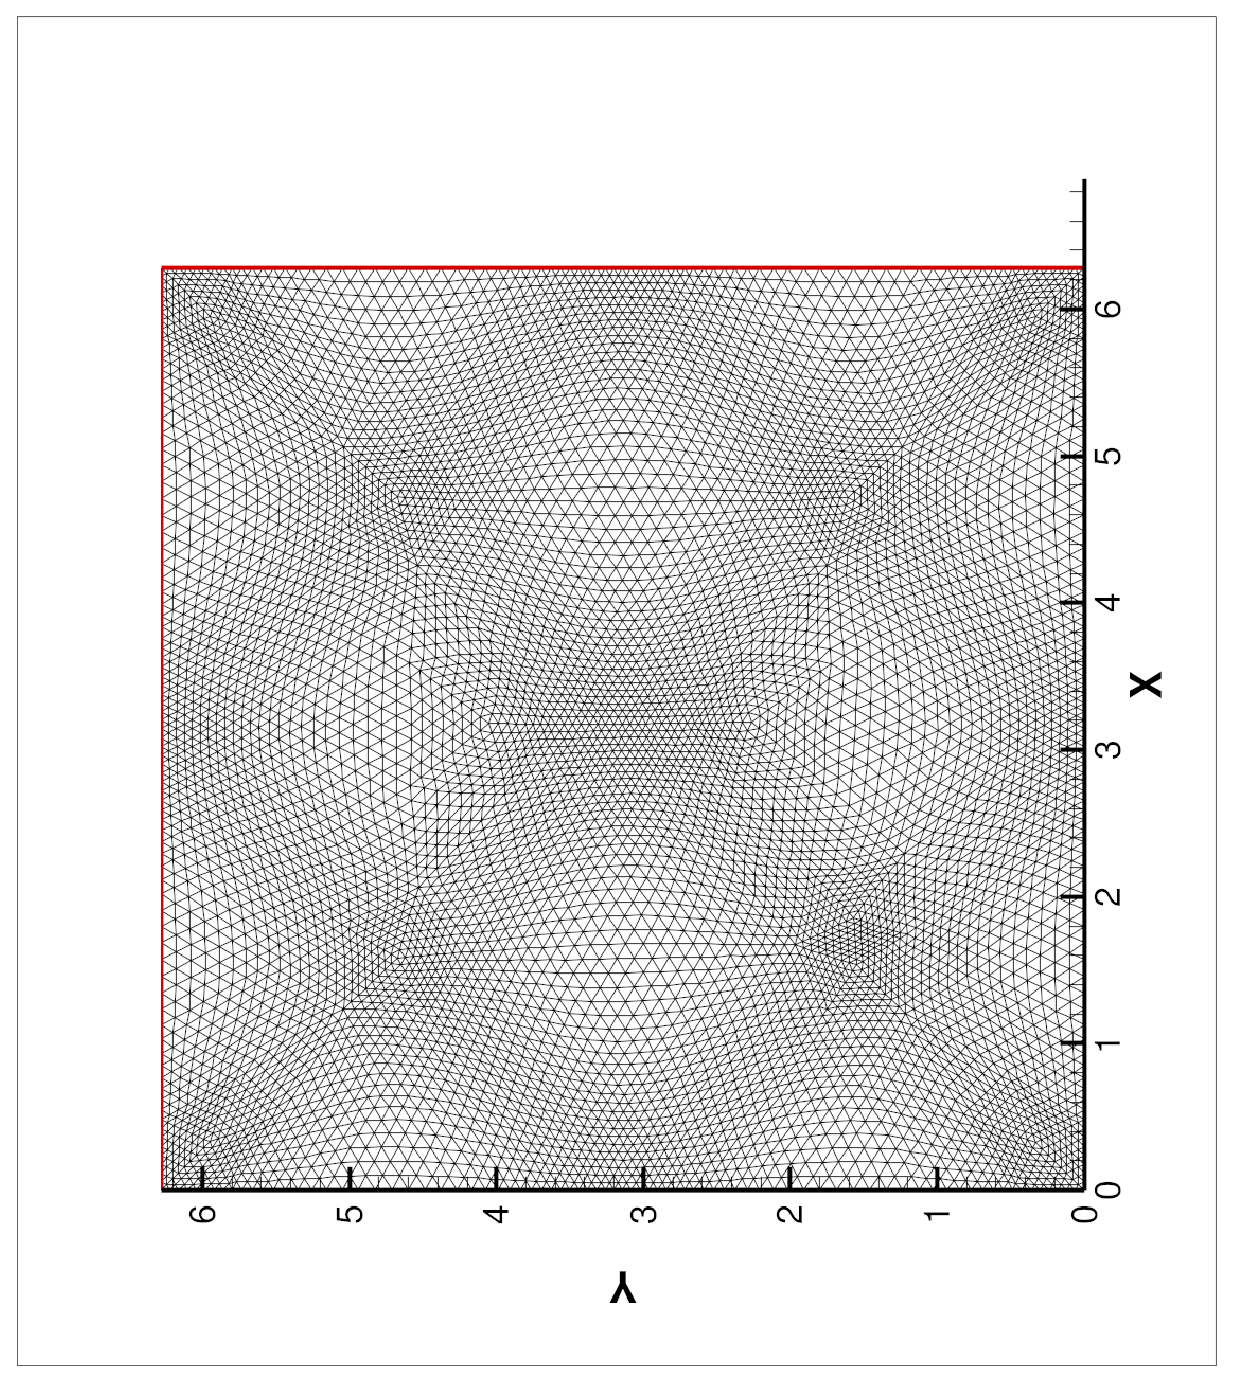
\includegraphics[width = 0.43\textwidth, angle = -90]{./moving40_meshV.eps}
   \caption{\small Moving mesh $40 \times 40$,
     Left: mesh P, right: mesh V, using monitor $G_1$
     in (\ref{eq::monitor_u_h}). $t = 1s, \nu = 0.05$.}
   \label{fig::moving40_mesh}
 \end{figure}

 From Figure(\ref{fig::moving40_monitor}), mesh is moving from the
 place where value of monitor is big to that which value is small.
 
 \begin{figure}[ht]
   \centering
   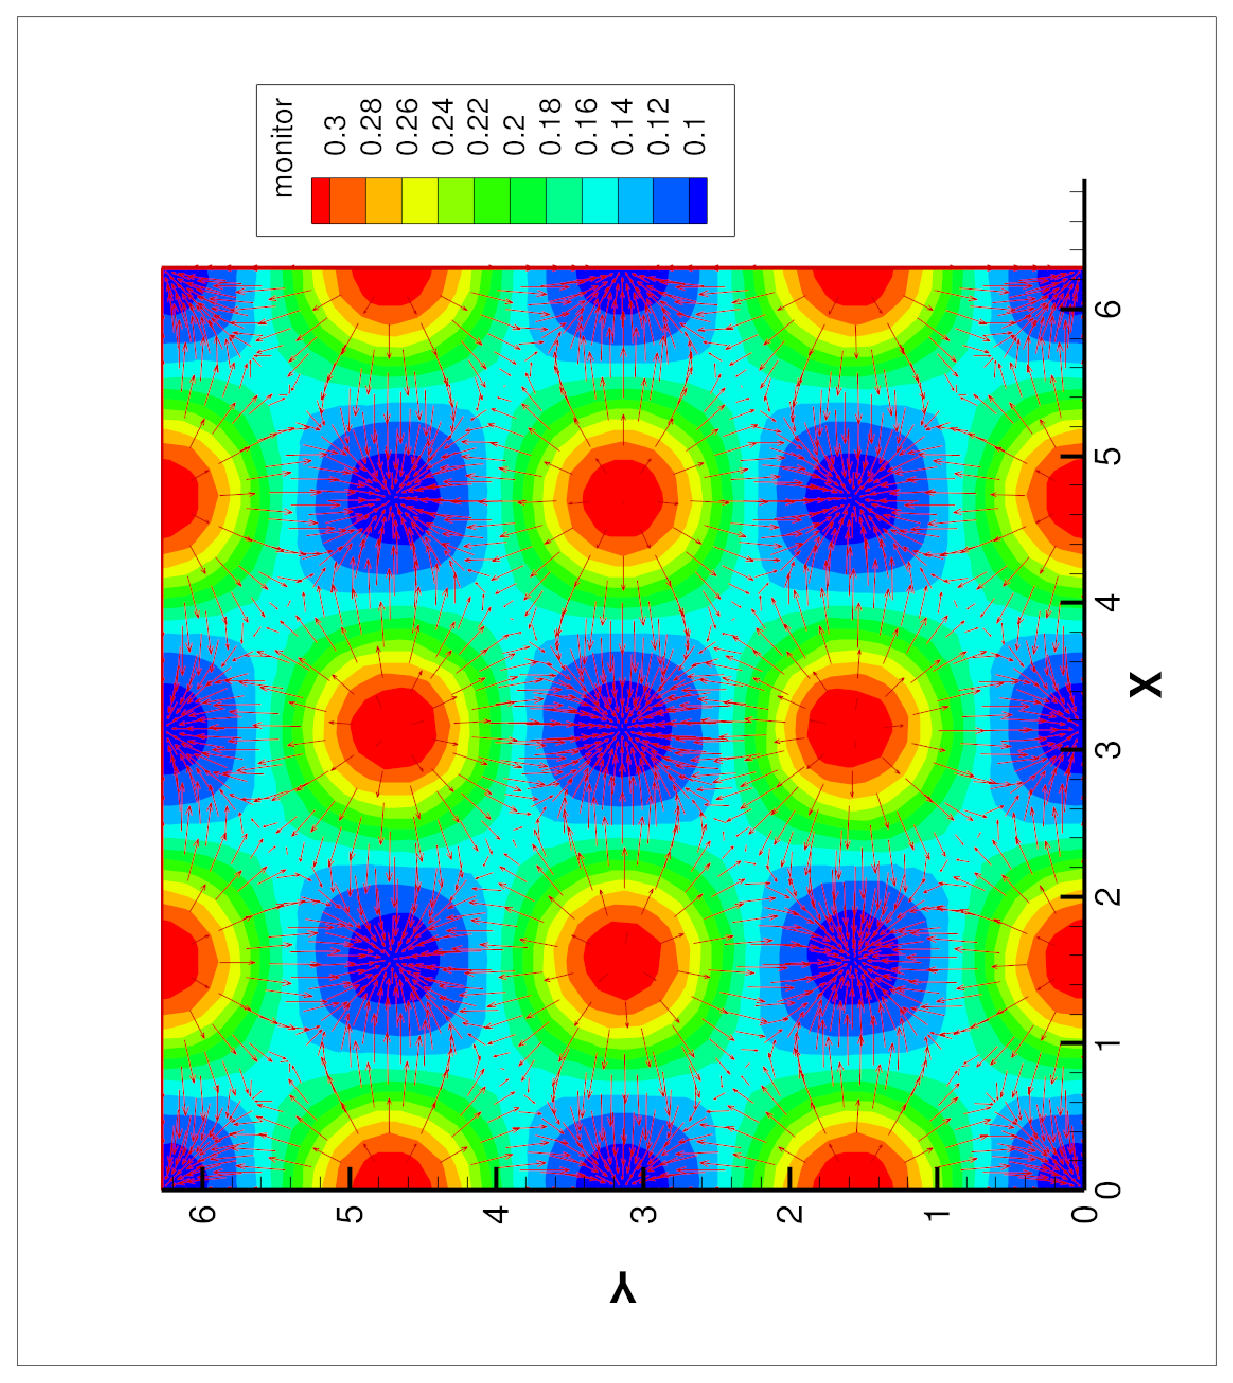
\includegraphics[width = 1.0\textwidth, angle = -90]{./moving40_movedirection.eps}
   \caption{\small Moving mesh $40 \times 40$,
     contour of monitor $m = \frac{1}{G_1}$ in (\ref{eq::monitor_u_h}).
     and mesh move direction. $t = 1s, \nu = 0.05$.}
   \label{fig::moving40_monitor}
 \end{figure}

% ----------------------------------------------------------------------------------------
%	SECTION 4
% ----------------------------------------------------------------------------------------

\section{Remarks}
% ----------------------------------------------------------------------------------------
%	BIBLIOGRAPHY
% ----------------------------------------------------------------------------------------

\bibliographystyle{plain}

\bibliography{sample, mathpaper, mathbook}
% ----------------------------------------------------------------------------------------


\end{document}
